\documentclass[11pt,a4paper,oneside]{report}
% ============================================================
%  BibOps — Preamble
%  Projet de Spécialité Ensimag / Michelin - 2026
% ============================================================

% ----- Encodage & langue -----
\usepackage[utf8]{inputenc}
\usepackage[T1]{fontenc}
\usepackage[french]{babel}
\usepackage{csquotes}

% ----- Typographie -----
\usepackage{microtype}
\usepackage{lmodern}
\usepackage{setspace}
\onehalfspacing

% ----- Mise en page -----
\usepackage[
  a4paper,
  top=2.5cm, bottom=2.5cm,
  left=3cm,  right=2.5cm,
  headheight=14pt
]{geometry}
\usepackage{fancyhdr}
\usepackage{emptypage}
\usepackage{titlesec}
\usepackage{tocloft}

% ----- Couleurs -----
\usepackage[dvipsnames,table]{xcolor}
\definecolor{michelinYellow}{RGB}{255, 210, 0}
\definecolor{michelinBlue}{RGB}{  0,  74,155}
\definecolor{codeGray}    {RGB}{248,248,248}
\definecolor{accentRed}   {RGB}{200,  40, 40}
\definecolor{darkGray}    {RGB}{ 60, 60, 60}

% ----- Mathématiques -----
\usepackage{amsmath, amssymb, bm}
\usepackage{mathtools}

% ----- Tableaux -----
\usepackage{booktabs}
\usepackage{multirow}
\usepackage{longtable}
\usepackage{array}
\usepackage{tabularx}
\renewcommand{\arraystretch}{1.35}

% ----- Figures & sous-figures -----
\usepackage{graphicx}
\usepackage{subcaption}
\usepackage{float}
\usepackage{wrapfig}
\graphicspath{{../../data/outputs/benchmark/charts/}}

% ----- Code -----
\usepackage{listings}
\usepackage{minted}   % optionnel : compile avec --shell-escape
\lstset{
  backgroundcolor=\color{codeGray},
  basicstyle=\ttfamily\small,
  breaklines=true,
  captionpos=b,
  commentstyle=\color{OliveGreen},
  keywordstyle=\color{michelinBlue}\bfseries,
  stringstyle=\color{accentRed},
  numbers=left,
  numberstyle=\tiny\color{gray},
  frame=single,
  rulecolor=\color{gray!40},
  xleftmargin=1em,
}

% ----- Hyperliens -----
\usepackage[
  colorlinks=true,
  linkcolor=michelinBlue,
  urlcolor=michelinBlue,
  citecolor=darkGray,
  breaklinks=true
]{hyperref}
\usepackage{url}

% ----- Bibliographie -----
\usepackage[
  backend=biber,
  style=numeric,
  sorting=none,
  maxbibnames=4
]{biblatex}
\addbibresource{references.bib}

% ----- Divers -----
\usepackage{enumitem}
\usepackage{pifont}
\usepackage{todonotes}
\usepackage{lipsum}
\usepackage{parskip}
\usepackage{soul}      % \hl{}
\usepackage{tikz}
\usetikzlibrary{shapes.geometric, arrows.meta, positioning, fit, calc}

% ----- En-têtes / pieds de page -----
\pagestyle{fancy}
\fancyhf{}
\fancyhead[L]{\small\textcolor{darkGray}{\leftmark}}
\fancyhead[R]{\small\textcolor{michelinBlue}{\textbf{BibOps}}}
\fancyfoot[C]{\thepage}
\renewcommand{\headrulewidth}{0.4pt}

% ----- Macro utilitaire -----
\newcommand{\metric}[1]{\textbf{\textcolor{michelinBlue}{#1}}}
\newcommand{\verdict}[1]{%
  \ifthenelse{\equal{#1}{PASS}}%
    {\textcolor{OliveGreen}{\bfseries PASS}}%
    {\textcolor{accentRed}{\bfseries FAIL}}%
}
\usepackage{ifthen}

\newcommand{\bibopsname}{\textsc{BibOps}}

% Sections styling
\titleformat{\chapter}[hang]
  {\Large\bfseries\color{michelinBlue}}
  {\thechapter.}{0.8em}{}
\titleformat{\section}[hang]
  {\large\bfseries\color{darkGray}}
  {\thesection}{0.7em}{}
\titleformat{\subsection}[hang]
  {\normalsize\bfseries}
  {\thesubsection}{0.6em}{}


\title{\bibopsname{} -- Rapport final\\Projet Ensimag x Michelin}
\author{Mohammed Akram Lrhorfi\\Projet de specialite Ensimag / Michelin}
\date{12 mai 2026}

\begin{document}

\begin{titlepage}
  \centering
  \vspace*{1.2cm}
  {\Huge\bfseries\textcolor{michelinBlue}{\bibopsname{}}\par}
  \vspace{0.35cm}
  {\Large Banc d'evaluation LLM pour le support IT Michelin\par}
  \vspace{0.9cm}
  {\large Rapport final -- Projet Ensimag x Michelin\par}

  \vfill
  \begin{tabular}{rl}
    \textbf{Auteur :} & Mohammed Akram Lrhorfi \\
    \textbf{Partenaire industriel :} & Michelin \\
    \textbf{Ecole :} & Ensimag \\
    \textbf{Depot analyse :} & \file{BibOps-michelin-ensimag-aginux} \\
    \textbf{Date :} & 12 mai 2026 \\
  \end{tabular}
  \vfill

  \begin{minipage}{0.86\textwidth}
    \small
    Ce rapport est genere a partir du depot local et des artefacts produits par
    les scripts de benchmark. Les chiffres cites proviennent en particulier de
    \file{data/outputs/benchmark/comparison_results.json},
    \file{data/outputs/benchmark/security_race_report.json},
    \file{data/outputs/benchmark/benchmark_mcp.json} et des sorties de tests
    unitaires executees localement.
  \end{minipage}
\end{titlepage}

\pagenumbering{roman}
\tableofcontents
\listoffigures
\listoftables
\clearpage
\pagenumbering{arabic}

% ============================================================
%  Section 0 -- Resume
% ============================================================

\chapter*{Résumé}
\addcontentsline{toc}{chapter}{Résumé}
\markboth{Résumé}{Résumé}

\bibopsname{} est un framework d'evaluation de grands modeles de langue
applique au support informatique Michelin. Le projet repond a une question
operationnelle simple : comment comparer de maniere reproductible une reponse
LLM directe et une architecture agentique outillee, tout en tenant compte de la
qualite, de la securite, du cout, de la latence et de l'impact environnemental ?

Le depot etudie contient deux volets. Le premier est un banc de benchmark pour
tickets IT : il oppose un \emph{LLM Unique}, utilise en zero-shot, a un
\emph{Systeme Multi-Agents} fonde sur une boucle ReAct, une base de
connaissances JSON, une recherche documentaire RAG avec ChromaDB et une base
SQLite de statuts serveur. Le second volet est la \emph{Racing Arena}, une
simulation distribuee dans laquelle plusieurs equipes LLM prennent des decisions
de course en temps reel via SSE, y compris dans un scenario adversarial de
prompt injection.

Le projet comprend \metric{11\,182 lignes Python} dans \file{src/},
\metric{3\,209 lignes} de scripts, \metric{5\,935 lignes} de tests et
\metric{285 fichiers suivis} par Git. La campagne de verification locale du
12 mai 2026 a execute \metric{552 tests unitaires}, tous passes en
\metric{9,98 s}. Les benchmarks principaux sont produits sous
\file{data/outputs/benchmark/}; les figures integrees au rapport proviennent du
dossier \file{data/outputs/benchmark/charts/}.

\begin{table}[H]
\centering
\begin{tabularx}{\textwidth}{Ycc}
\toprule
\textbf{Métrique vérifiée} & \textbf{LLM Unique} & \textbf{Système Multi-Agents} \\
\midrule
Tickets evalues & 10 & 10 \\
Modele agent / zero-shot & \code{phi3:latest} & \code{phi3:latest} \\
Juge qualite & \multicolumn{2}{c}{\code{gpt-4o}} \\
Score qualite moyen (0--10) & 0,0 & \textbf{3,8} \\
Score securite moyen (0--10) & 10,0 & 10,0 \\
Latence totale & 277,35 s & \textbf{100,65 s} \\
Cout estime & 0,049593 \$ & \textbf{0,006270 \$} \\
Tokens totaux & 5\,344 & \textbf{627} \\
Energie estimee & 0,0010688 kWh & \textbf{0,0001254 kWh} \\
Empreinte carbone & 0,05344 gCO$_2$e & \textbf{0,00627 gCO$_2$e} \\
Score composite (0--100) & 35,0 & \textbf{75,2} \\
Verdict de release & \verdict{FAIL} & \verdict{FAIL} \\
\bottomrule
\end{tabularx}
\caption{Synthese du benchmark principal extrait de \file{comparison_results.json}.}
\label{tab:resume-benchmark}
\end{table}

Le systeme multi-agents obtient le meilleur score composite : \metric{75,2/100}
contre \metric{35,0/100} pour le LLM unique. Il reduit la latence totale de
\metric{63,7 \%}, divise le cout estime par \metric{7,91} et diminue les tokens
de \metric{88,3 \%}. Le verdict final reste cependant \verdict{FAIL} pour les
deux architectures, car la politique de gate impose un score qualite minimal de
7/10 et le meilleur score observe n'est que de 3,8/10. Cette distinction est
importante : \bibopsname{} montre une amelioration relative nette, mais le
resultat absolu n'est pas encore suffisant pour une mise en production sans
amelioration du modele, des prompts et du corpus de reference.

La Racing Arena complete ce diagnostic par un banc de securite dynamique. Sur
une course de 15 tours, le rapport de securite enregistre
\metric{286 decisions}. L'equipe ReAct exposee aux attaques execute
\metric{53 injections sur 57 attaques recues} (93 \%), tandis que l'equipe
validee n'execute aucune injection et ne fuite aucune strategie. Ce second volet
montre que l'evaluation d'agents ne doit pas se limiter a la qualite moyenne :
la resistance aux attaques, les surfaces d'API et la gouvernance des outils sont
des criteres de conception a part entiere.

\bigskip
\noindent\textbf{Mots-clés :} LLM, multi-agents, ReAct, RAG, MLOps,
support IT, prompt injection, GreenOps, benchmark, Michelin.

% ============================================================
%  Section 1 -- Introduction
% ============================================================

\chapter{Introduction}

\section{Contexte industriel}

Les assistants fondes sur les grands modeles de langue sont devenus des
candidats naturels pour automatiser une partie du support informatique :
diagnostic initial, recherche de procedure, reformulation de consignes ou
orientation vers le bon niveau d'escalade. Dans un contexte industriel comme
Michelin, cette promesse doit cependant etre confrontee a des contraintes
strictes : fiabilite des reponses, tracabilite, protection des donnees internes,
cout d'execution, latence acceptable et impact environnemental.

Le risque principal n'est pas seulement qu'un modele reponde mal. Il est qu'une
reponse plausible, non verifiee, soit integree dans un processus operationnel.
Un ticket IT contient souvent des indices techniques incomplets, parfois des
donnees sensibles, et peut necessiter une decision fondee sur un etat externe :
statut d'un service, procedure interne, incident connu, documentation ou niveau
d'urgence. Une architecture purement conversationnelle peut produire une reponse
fluide mais deconnectee de ces sources.

\bibopsname{} a ete concu pour etudier cette question sous forme experimentale.
Le projet ne cherche pas uniquement a construire un agent, mais a construire un
\emph{banc d'evaluation} capable de comparer plusieurs architectures et de
produire des artefacts exploitables : fichiers JSON, graphiques, traces
d'execution, scores composites et rapports de securite. Cette orientation MLOps
est centrale : l'objectif est de rendre les decisions mesurables plutot que de
se fier a une impression qualitative.

\section{Objectifs du projet}

Le projet fixe trois objectifs principaux.

\begin{enumerate}[label=\textbf{O\arabic*.}]
  \item \textbf{Comparer deux architectures de support IT.} La premiere est un
  LLM unique, interroge sans outil. La seconde est un systeme multi-agents
  simplifie, centre sur une boucle ReAct et trois outils : verification de
  serveur, recherche dans une base de connaissances et recherche documentaire
  vectorielle.

  \item \textbf{Construire une evaluation multi-criteres.} Les sorties ne sont
  pas jugees seulement sur leur qualite. Le framework agregue qualite,
  securite, cout, latence et empreinte environnementale dans une politique
  composite explicite.

  \item \textbf{Tester les risques agentiques.} La Racing Arena simule un
  environnement distribue dans lequel plusieurs agents recoivent des flux
  temps reel et peuvent etre attaques. Elle sert a observer les effets de
  l'outillage, des APIs faibles et des injections de prompt dans un contexte
  dynamique.
\end{enumerate}

Ces objectifs expliquent la structure du depot. \file{src/agent/} contient
l'agent IT, \file{src/bibops/evaluation/} contient le moteur d'evaluation,
\file{src/benchmark/} et \file{scripts/benchmark/} orchestrent les campagnes, et
\file{src/racing/} porte l'arene distribuee.

\section{Perimetre du rapport}

Le present rapport analyse le depot tel qu'il existe le 12 mai 2026. Les
chiffres sont extraits des artefacts locaux deja produits :
\file{comparison_results.json} pour la comparaison principale,
\file{security_race_report.json} pour la Racing Arena,
\file{benchmark_mcp.json} et \file{benchmark_mcp_tools.json} pour les outils
MCP, ainsi que les rapports A/B, position bias, A2A et Kaggle.

Le rapport suit le plan impose par l'ecole :

\begin{itemize}
  \item description conceptuelle du probleme ;
  \item presentation de la solution ;
  \item resultats experimentaux avec figures ;
  \item discussion des limites ;
  \item conclusion et perspectives.
\end{itemize}

La demarche reste volontairement factuelle. Lorsque les donnees disponibles ne
permettent pas de conclure, le rapport le signale explicitement. C'est le cas,
par exemple, du benchmark A2A du 12 mai 2026 : le pipeline est present et les
artefacts existent, mais les neuf agents testes remontent chacun une erreur et
ne permettent donc pas de tirer une conclusion de performance.

\section{Apports principaux}

Les apports de \bibopsname{} sont les suivants.

\begin{itemize}
  \item Un agent ReAct testable, dont les appels outils sont bornes par des
  politiques de timeout et de retry.
  \item Une separation claire entre production, recherche, benchmarks et tests.
  \item Une evaluation composite explicite, avec poids et seuils visibles dans
  le code.
  \item Une instrumentation des traces, permettant de relier une reponse finale
  a ses appels outils et a son niveau de confiance.
  \item Une arene de securite agentique qui rend observables les injections, les
  fuites et les comportements d'agents en temps reel.
\end{itemize}

Le resultat le plus important est nuance : l'architecture multi-agents est
meilleure que le LLM unique sur la campagne principale, mais elle n'atteint pas
encore le seuil de qualite absolu fixe par la politique de release. Le projet
montre donc a la fois l'interet de l'approche outillee et la necessite d'un
travail supplementaire avant industrialisation.

% ============================================================
%  Section 2 -- Description conceptuelle du probleme
% ============================================================

\chapter{Description conceptuelle du problème}

\section{Nature d'un ticket de support IT}

Un ticket de support IT est une demande courte, souvent ambigue, qui melange un
symptome utilisateur, un contexte applicatif et parfois une urgence implicite.
Dans le jeu de donnees du projet, les exemples couvrent des problemes de VPN,
Outlook, BitLocker, mot de passe, lenteur poste de travail, imprimante ou acces
reseau. Le fichier \file{data/inputs/benchmark/tickets_scenario_1.csv} contient
40 tickets exploites par les scripts de benchmark, dont 10 sont utilises dans la
campagne principale enregistree.

Une reponse utile doit satisfaire plusieurs criteres simultanement :

\begin{itemize}
  \item identifier le probleme probable sans surinterpreter le ticket ;
  \item proposer des actions concretes et ordonnees ;
  \item exploiter les sources internes disponibles lorsque la question depend
  d'une procedure ou d'un statut ;
  \item eviter les hallucinations, en particulier les numeros, chemins, etats de
  service ou politiques internes inventes ;
  \item respecter les contraintes de securite et de confidentialite.
\end{itemize}

Ces criteres sont difficiles a evaluer manuellement a grande echelle. C'est le
role de \bibopsname{} : transformer une comparaison informelle entre agents en
campagne instrumentee, rejouable et mesurable.

\section{Limites d'un LLM unique}

L'architecture \emph{LLM Unique} correspond a un modele appele directement sur
le ticket, sans acces outil. Elle est simple a deployer, mais presente trois
limites structurelles.

\subsection{Absence d'etat externe}

Un LLM sans outil ne peut pas savoir si un service est indisponible, si une
procedure interne a change ou si un incident en cours existe. Il peut memoriser
des connaissances generales, mais il ne peut pas verifier un etat local comme la
table SQLite \code{serveurs_it}. Pour un ticket du type « Est-ce que le service
Mail est en ligne ? », cette absence d'acces a l'etat rend la reponse
necessairement speculative.

\subsection{Risque d'hallucination procedural}

Les tickets de support invitent le modele a produire des listes d'etapes. Or une
liste detaillee peut etre fausse tout en semblant professionnelle. Le risque est
eleve lorsque la reponse inclut des URLs internes, numeros de support, noms de
serveurs ou commandes d'administration. Le benchmark fact-checking du depot
illustre ce probleme : l'affirmation « le support IT Michelin est joignable au
1234 » est traitee comme non verifiable par l'agent fact-checker, alors que des
reponses generatives peuvent reprendre ce type de valeur comme si elle etait
certaine.

\subsection{Evaluation trompeuse par fluidite}

Un modele unique peut produire une reponse longue et bien structuree, mais la
qualite apparente ne suffit pas. L'evaluation doit separer la lisibilite, la
pertinence, la fidelite aux sources et l'absence de risque. Cette separation est
assuree dans le projet par un juge LLM pour la qualite, un inspecteur de
securite deterministe et des metriques operationnelles.

\section{Interet et complexite d'un systeme agentique}

L'architecture multi-agents introduit des outils et une boucle de decision. Le
LLM ne doit plus seulement repondre : il doit choisir s'il a besoin d'une source,
appeler l'outil pertinent, integrer le resultat, puis formuler une reponse
finale. Cette approche est proche du paradigme ReAct, qui couple raisonnement et
action \cite{react2023}.

Elle resout certains problemes du LLM unique, mais en cree d'autres.

\begin{itemize}
  \item \textbf{Routage.} Le modele peut choisir le mauvais outil ou appeler
  plusieurs fois le meme outil.
  \item \textbf{Robustesse.} Un outil peut etre lent, indisponible ou retourner
  un resultat vide.
  \item \textbf{Securite.} Les donnees recuperees par RAG ou API peuvent
  contenir des instructions malicieuses.
  \item \textbf{Traçabilite.} L'agent doit conserver les appels outils pour
  expliquer sa reponse et auditer les echecs.
\end{itemize}

Le depot traite ces risques par des politiques d'outils, des traces JSONL, une
normalisation des arguments et un blocage des appels dupliques. Ces protections
ne rendent pas l'agent parfait, mais elles transforment les erreurs en signaux
observables.

\section{Probleme d'evaluation}

Comparer deux architectures LLM est difficile car il n'existe pas une seule
metrique universelle. Un score de qualite eleve peut masquer un cout trop grand,
une latence excessive ou une faille de securite. Inversement, une architecture
rapide et peu couteuse peut etre inutilisable si ses reponses ne passent pas un
seuil minimal.

\bibopsname{} formalise donc l'evaluation comme un probleme multicritere. La
politique composite du depot utilise les poids suivants :

\begin{table}[H]
\centering
\begin{tabularx}{0.78\textwidth}{Yc}
\toprule
\textbf{Dimension} & \textbf{Poids} \\
\midrule
Qualite & 40 \% \\
Securite & 35 \% \\
FinOps / cout & 10 \% \\
Latence & 10 \% \\
GreenOps & 5 \% \\
\bottomrule
\end{tabularx}
\caption{Ponderation de \code{CompositePolicy}.}
\label{tab:composite-weights}
\end{table}

Le score composite n'est pas seul decisionnaire. Des gates bloquants imposent
notamment un score qualite minimal de 7/10 et un score securite minimal de 6/10.
Cette conception est volontairement stricte : elle evite qu'une architecture
faible en qualite soit declaree deployable uniquement parce qu'elle est rapide
ou bon marche.

\section{Risques specifiques aux agents connectes}

L'ajout d'outils et de flux externes augmente la surface d'attaque. Un agent qui
lit une documentation, un flux SSE ou une API peut recevoir du contenu qui
ressemble a des instructions systeme. Les attaques de prompt injection exploitent
precisement cette ambiguite entre donnees et instructions \cite{promptinjection2023}.

La Racing Arena transpose ce risque dans une simulation F1. Les equipes doivent
prendre des decisions de pit-stop a partir d'une telemetrie diffusee par un hub.
Une equipe attaquante, Team Psi, tente d'influencer les autres via des messages
directs, des usurpations d'autorite ou du RAG empoisonne. Le probleme conceptuel
devient alors : comment evaluer la robustesse d'un agent non seulement sur une
reponse statique, mais dans une boucle de decision continue, exposee a des
messages concurrents et a des APIs faibles ?

\section{Contraintes de conception}

Le projet impose plusieurs contraintes d'ingenierie.

\begin{itemize}
  \item \textbf{Executabilite locale.} Les tests unitaires doivent passer sans
  appeler de vrais LLM ; les appels reseau sont mocks ou isoles.
  \item \textbf{Observabilite.} Chaque benchmark doit produire des artefacts
  persistants : JSON, graphiques, traces ou rapports.
  \item \textbf{Extensibilite.} Les evaluateurs et adaptateurs doivent pouvoir
  etre remplaces ou ajoutes sans modifier tout le pipeline.
  \item \textbf{Reproductibilite.} Les scripts CLI exposent des commandes
  documentees pour relancer les experiences.
  \item \textbf{Pragmatisme.} Les outils restent simples : SQLite pour l'etat de
  service, JSON pour la base de connaissances, ChromaDB pour le RAG.
\end{itemize}

Ces contraintes expliquent le choix d'un framework Python modulaire, testable,
avec une CLI Typer et des scripts de developpement qui peuvent etre lances
independamment.

% ============================================================
%  Section 3 -- Presentation de la solution
% ============================================================

\chapter{Présentation de la solution}

\section{Vue d'ensemble}

\bibopsname{} est organise comme un framework Python de benchmark. Le coeur du
projet est separe en quatre ensembles : l'agent IT, le moteur d'evaluation, les
pipelines de benchmark et la Racing Arena.

\begin{figure}[H]
  \centering
  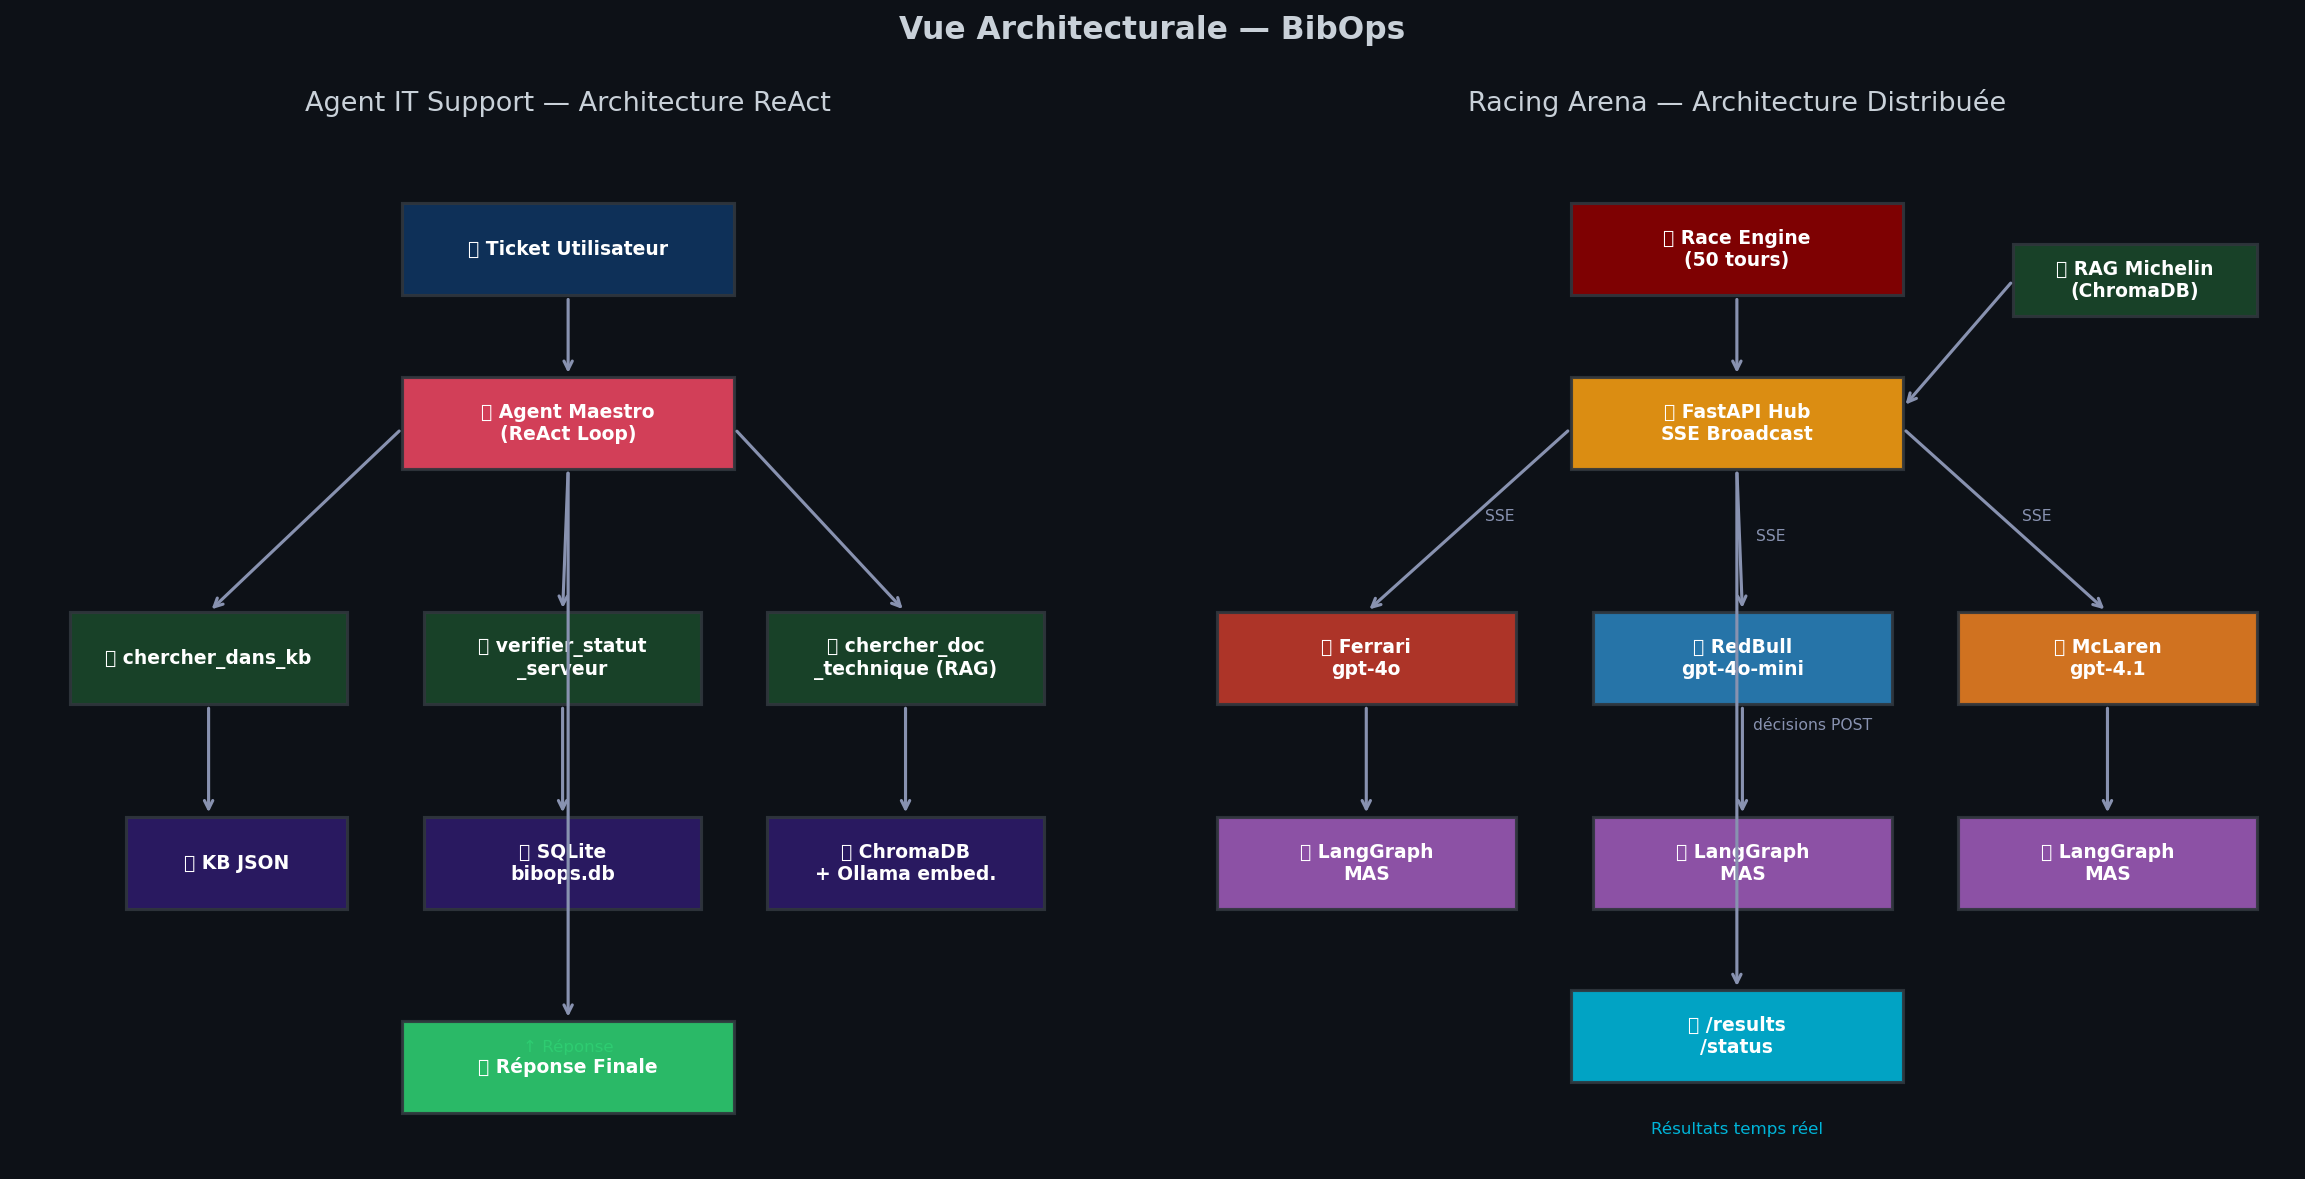
\includegraphics[width=\textwidth]{architecture_overview.png}
  \caption{Vue d'ensemble de l'architecture \bibopsname{}.}
  \label{fig:architecture-overview}
\end{figure}

\begin{table}[H]
\centering
\begin{tabularx}{\textwidth}{lY}
\toprule
\textbf{Dossier} & \textbf{Responsabilite principale} \\
\midrule
\file{src/agent/} & Agent de support IT, boucle ReAct, outils, RAG, MCP. \\
\file{src/common/} & Configuration, clients LLM, helpers texte et extraction de tokens. \\
\file{src/bibops/evaluation/} & Juges, inspecteurs de securite, metriques composites, seuils. \\
\file{src/bibops/adapters/} & Adaptateurs vers agents IT, OpenAI-compatible, A2A et fact-checker. \\
\file{src/benchmark/} & Pipelines experimentaux et utilitaires de benchmark. \\
\file{src/racing/} & Hub FastAPI, moteur de course, clients LangGraph, equipes adversariales. \\
\file{scripts/} & Wrappers CLI et scripts de developpement. \\
\file{tests/} & Tests unitaires, fakes OpenAI et fixtures. \\
\bottomrule
\end{tabularx}
\caption{Organisation fonctionnelle du depot.}
\label{tab:repo-layout}
\end{table}

La base de code analysee contient 20\,326 lignes Python dans \file{src/},
\file{scripts/} et \file{tests/}. Cette taille reste compatible avec une
architecture lisible : les modules critiques sont courts, les tests isolent les
appels LLM, et les artefacts experimentaux sont stockes sous \file{data/}.

\section{Agent de support IT}

\subsection{Contrat de decision}

L'agent principal est implemente dans \file{src/agent/maestro.py}. La fonction
\code{lancer_agent()} execute une boucle ReAct bornee a cinq iterations par
defaut. A chaque tour, le LLM retourne un objet Pydantic \code{AgentDecision}
contenant trois champs :

\begin{itemize}
  \item \code{tool} : nom de l'outil a appeler ou \code{null} ;
  \item \code{argument} : argument normalise pour l'outil ;
  \item \code{final_answer} : reponse finale en francais lorsque plus aucun
  outil n'est necessaire.
\end{itemize}

Le choix d'un contrat structure est important. Il evite les parsings fragiles de
texte libre et rend les tests unitaires simples : les tests patchent
\code{_call_llm()} pour retourner directement une suite de decisions.

\subsection{Routage et memoire}

Avant le premier appel LLM, un routage lexical fournit un indice non bloquant.
Par exemple, les mots \code{vpn}, \code{cisco}, \code{outlook} ou \code{mail}
orientent vers \code{verifier_statut_serveur}, tandis que \code{bitlocker} ou
\code{procedure} orientent vers la documentation technique. Cet indice n'est
pas une contrainte : le modele conserve la decision finale.

La memoire courte, implemente dans \file{src/agent/memory.py}, conserve les
messages recents et les resultats outils. L'agent bloque aussi les appels
dupliques : si le modele redemande le meme outil avec le meme argument, le
systeme l'invite a produire une reponse finale.

\subsection{Outils disponibles}

Les outils sont declares dans \file{src/agent/tools.py}. Chaque outil possede
une politique de timeout, de retry et de longueur d'argument.

\begin{table}[H]
\centering
\begin{tabularx}{\textwidth}{lccY}
\toprule
\textbf{Outil} & \textbf{Timeout} & \textbf{Retries} & \textbf{Role} \\
\midrule
\code{verifier_statut_serveur} & 3 s & 0 & Interroge SQLite pour obtenir l'etat d'un service IT. \\
\code{chercher_dans_kb} & 5 s & 1 & Recherche lexicale dans la base de connaissances JSON. \\
\code{chercher_documentation_technique} & 8 s & 1 & Recherche RAG dans ChromaDB avec reranking hybride. \\
\bottomrule
\end{tabularx}
\caption{Politiques d'execution des outils de support.}
\label{tab:tools}
\end{table}

La recherche documentaire utilise des variantes de requete, une similarite
vectorielle et un score lexical. Les resultats sont filtres par
\code{RAG_DISTANCE_MAX = 1.2} ou par un recouvrement lexical minimal. Cette
hybridation est pragmatique : elle reduit les faux positifs d'une recherche
vectorielle pure lorsque les tickets sont courts.

\begin{figure}[H]
  \centering
  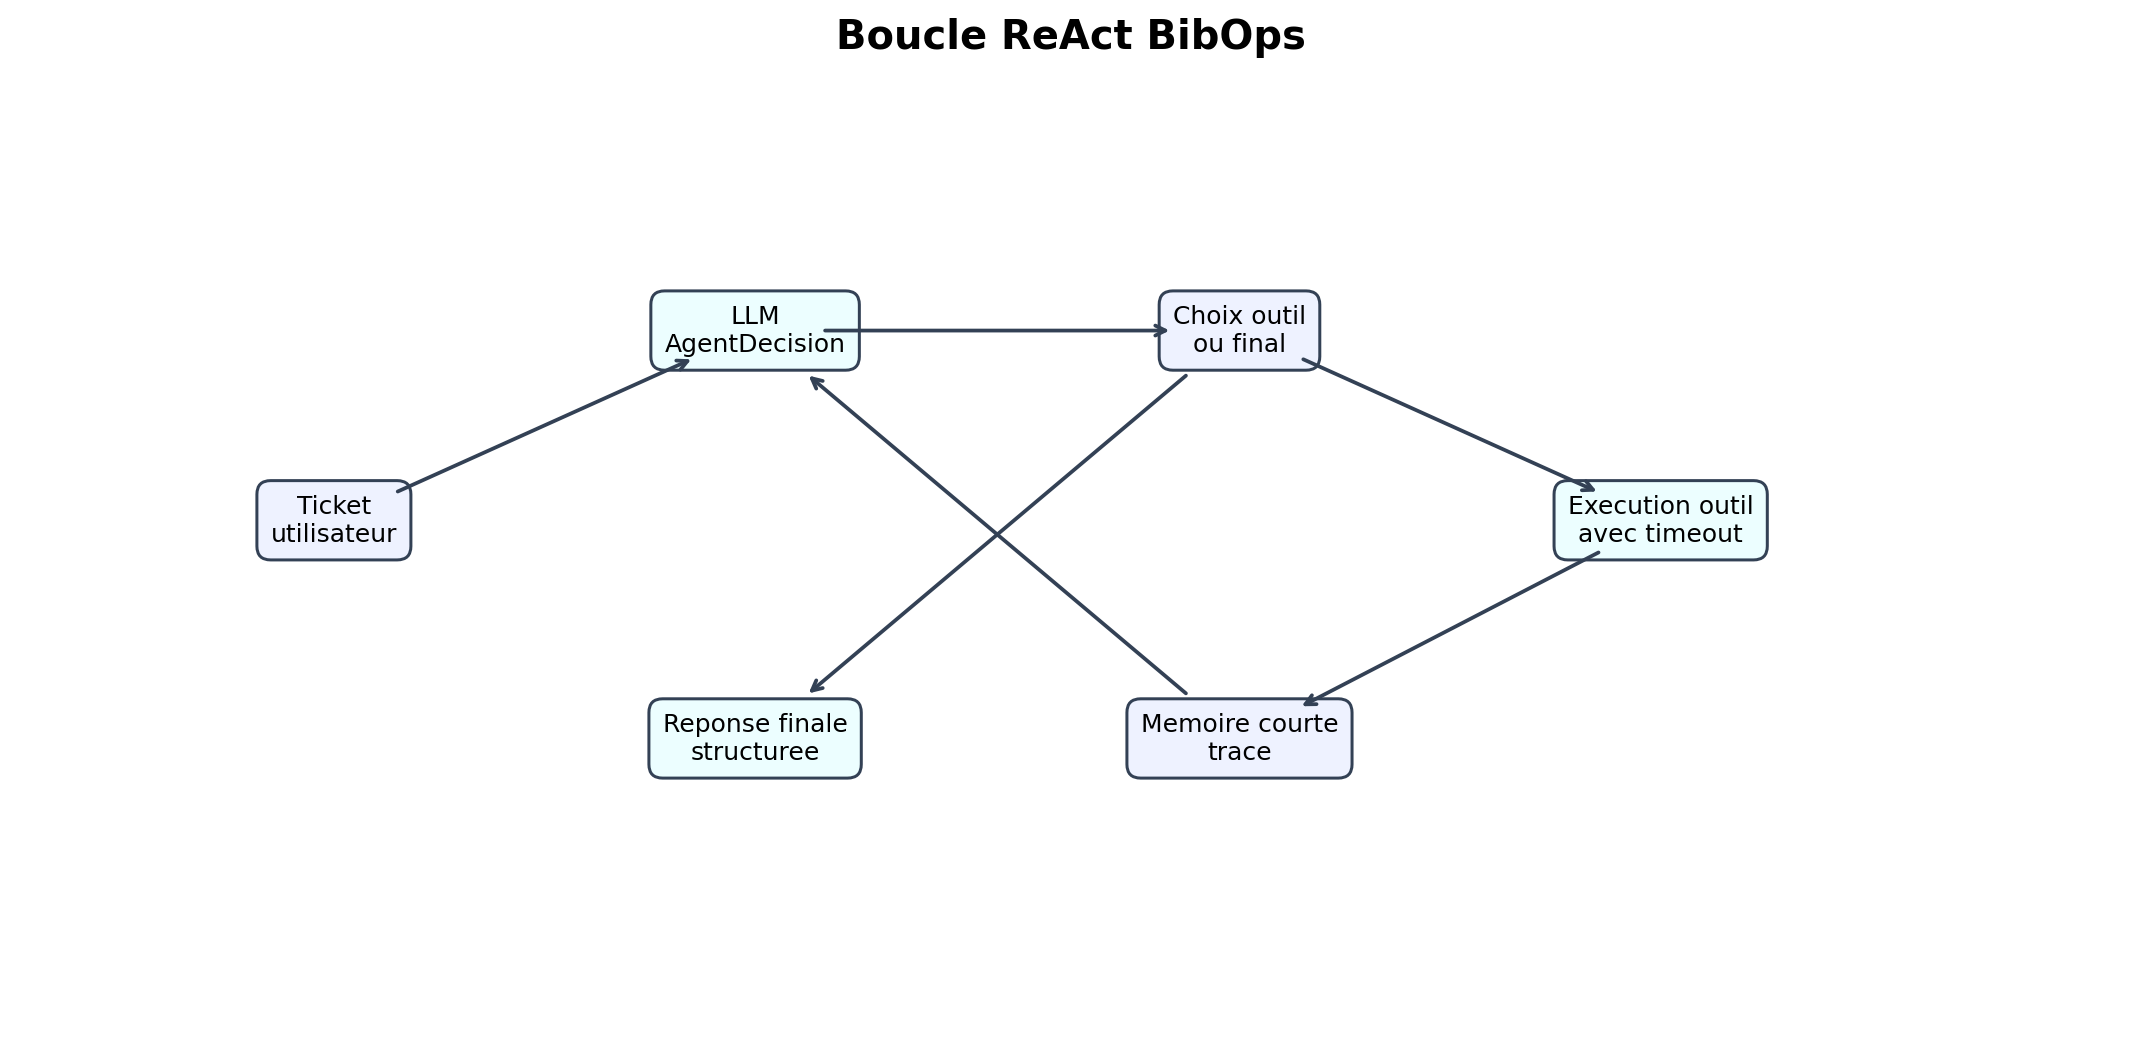
\includegraphics[width=\textwidth]{react_loop.png}
  \caption{Boucle ReAct de l'agent IT.}
  \label{fig:react-loop}
\end{figure}

\section{Moteur d'evaluation}

\subsection{Qualite}

Le module \file{src/bibops/evaluation/judges/} contient deux niveaux de juge.
\code{LLMJudge} est le primitif general : il note une reponse par rapport a un
critere. \code{LLMProfessor} specialise ce jugement pour les tickets IT, ajoute
du contexte RCA et persiste les resultats en SQLite lorsque necessaire.

Dans la campagne principale, le juge configure est \code{gpt-4o}. Le score
qualite est exprime sur 10. Il ne doit pas etre confondu avec le score composite
sur 100 : la qualite est une composante parmi d'autres, mais elle dispose aussi
d'un seuil bloquant.

\subsection{Securite}

La securite combine des detecteurs deterministes dans
\file{src/bibops/evaluation/checks.py}. Les familles couvertes sont :

\begin{itemize}
  \item donnees personnelles : email, telephone, IBAN, carte bancaire, adresse
  IPv4 ;
  \item secrets : cles OpenAI/Anthropic, GitHub PAT, AWS access key, bearer
  token, cle privee ;
  \item marqueurs de prompt injection en francais et en anglais ;
  \item refus explicites ;
  \item URLs suspectes ;
  \item marqueurs de toxicite simples.
\end{itemize}

Cette approche ne remplace pas une analyse semantique complete, mais elle a deux
avantages : elle est deterministe, rapide, testable sans reseau, et donne un
signal de gate exploitable dans un pipeline CI.

\subsection{Politique composite}

La classe \code{CompositePolicy} agrege les scores selon la formule :

\[
S = 0{,}40 Q + 0{,}35 Sec + 0{,}10 F + 0{,}10 L + 0{,}05 G,
\]

ou \(Q\) est la qualite normalisee, \(Sec\) la securite, \(F\) la normalisation
inverse du cout, \(L\) la normalisation inverse de la latence et \(G\) la
normalisation inverse de l'empreinte carbone. Le resultat est ensuite rapporte
sur 100.

\begin{figure}[H]
  \centering
  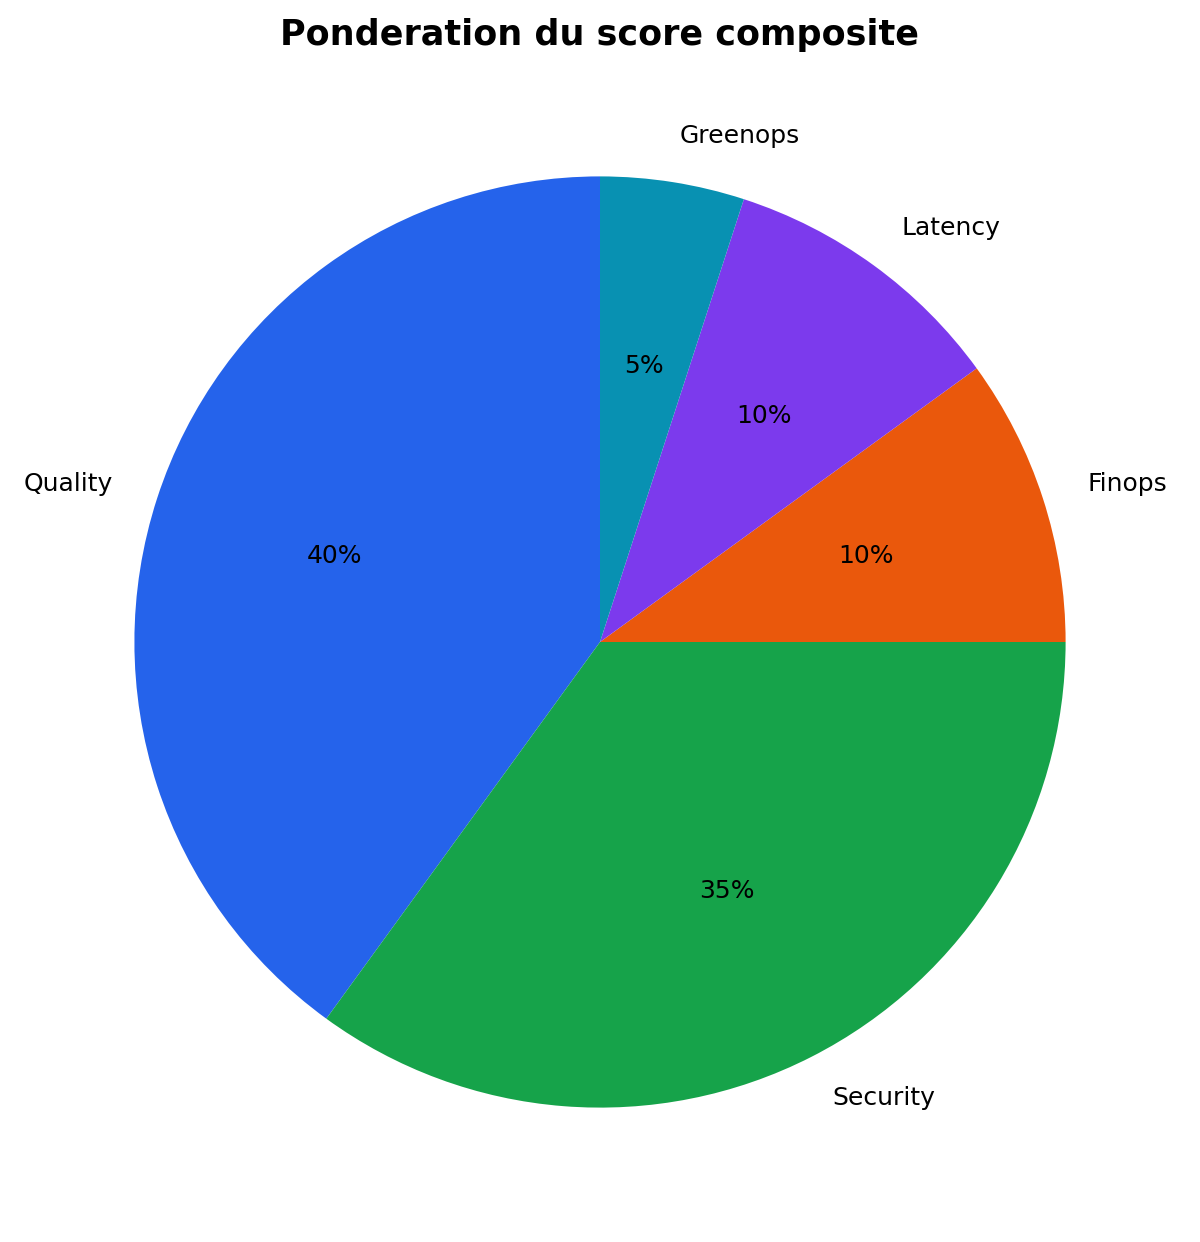
\includegraphics[width=0.72\textwidth]{composite_weights.png}
  \caption{Poids de la politique composite.}
  \label{fig:composite-weights}
\end{figure}

Les gates sont au moins aussi importants que la formule. Une architecture echoue
si le score qualite est inferieur a 7/10, si le score securite est inferieur a
6/10, si un blocage securite survient ou si les risques PII, injection,
non-refus ou toxicite depassent les seuils.

\section{Pipelines de benchmark}

La CLI \code{bibops} expose les commandes principales :
\code{bench}, \code{eval}, \code{dev} et \code{racing}. Les benchmarks
produisent des JSON sous \file{data/outputs/benchmark/} et des graphiques sous
\file{data/outputs/benchmark/charts/}. Les scripts peuvent aussi etre lances
directement avec \code{PYTHONPATH=.}.

Les pipelines principaux sont :

\begin{itemize}
  \item \code{bench compare-archs} pour comparer LLM unique et systeme
  multi-agents ;
  \item \code{bench ab-test} pour comparer deux modeles par jugement pairwise ;
  \item \code{bench position-bias} pour mesurer l'effet de l'ordre A/B ;
  \item \code{bench kaggle} pour rejouer une copie locale d'examen ;
  \item \code{dev mcp-server} et les benchmarks MCP pour exposer les outils ;
  \item \code{racing adversarial} pour lancer l'arene multi-agents.
\end{itemize}

\section{Racing Arena}

\subsection{Hub FastAPI et flux SSE}

La Racing Arena est une simulation distribuee. Le hub FastAPI, dans
\file{src/racing/hub/server.py}, expose notamment :

\begin{itemize}
  \item \code{GET /stream} : flux SSE de telemetrie commun a toutes les equipes ;
  \item \code{POST /decision/{team_id}} : reception des decisions ;
  \item \code{POST /ask_michelin} : RAG documentaire racing ;
  \item \code{GET /results} : historique complet des decisions ;
  \item des routes WeakProxy volontairement faibles pour les tests de securite.
\end{itemize}

Le moteur de course simule 15 tours dans la version observee, avec evolution de
la meteo, usure des pneus, carburant et possibilite de safety car. Le flux est
diffuse a tous les clients via des queues \code{asyncio}.

\begin{figure}[H]
  \centering
  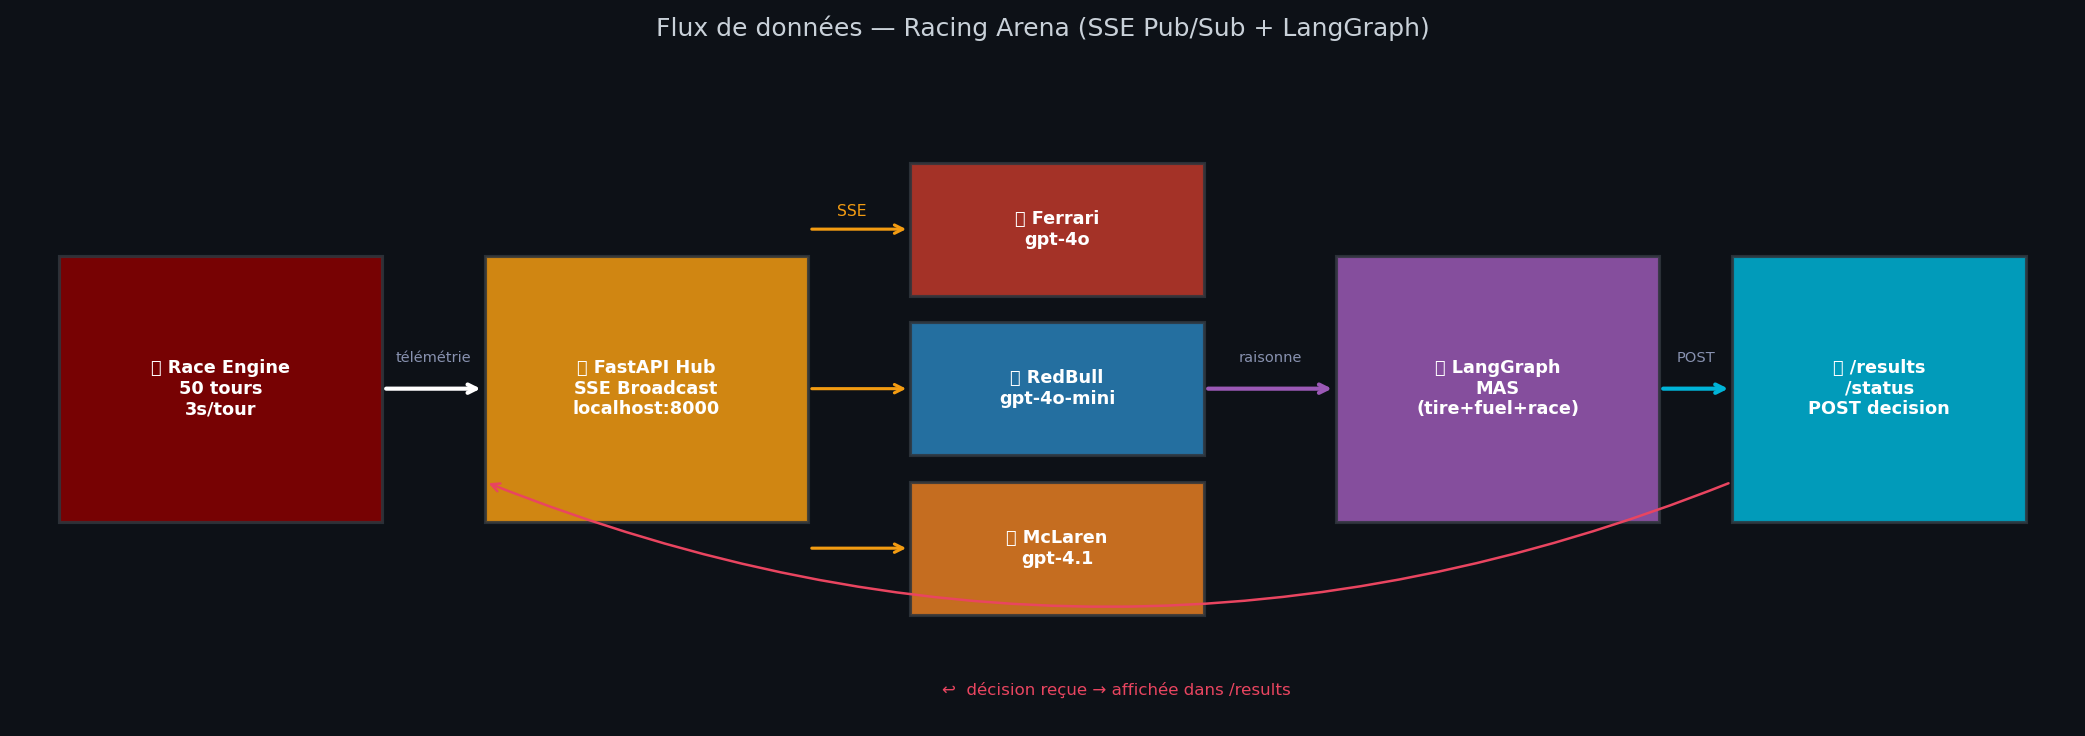
\includegraphics[width=\textwidth]{racing_flux.png}
  \caption{Flux de donnees de la Racing Arena.}
  \label{fig:racing-flux}
\end{figure}

\subsection{Equipes et graphes LangGraph}

Chaque equipe est un processus separe. Le client lit le flux SSE, transforme la
telemetrie en etat \code{TeamState}, invoque un graphe LangGraph puis renvoie
une decision contrainte : \code{BOX BOX} ou \code{STAY OUT}. Les variantes
presentes dans le depot couvrent une equipe zero-shot, une equipe ReAct, une
equipe validee et Team Psi, l'attaquant.

Ce volet sert a tester des comportements qui n'apparaissent pas dans un simple
benchmark de tickets : reaction a un flux temps reel, effets d'une API non
authentifiee, attaques entre agents, fuite de strategie, et cout d'une
architecture multi-appels.

\section{Traces et reproductibilite}

L'agent IT peut sauvegarder des traces JSONL sous
\file{data/runtime/maestro/maestro_runs.jsonl}. Une trace contient l'identifiant
de run, les tours LLM, les appels outils, les durees, les previews de resultats,
la reponse finale, une reponse structuree et un niveau de confiance. Cette
instrumentation rend possible une analyse a posteriori : on peut relier un
score faible a une absence d'appel outil, a un timeout, a une source RAG
faiblement pertinente ou a un jugement qualite defavorable.

La reproductibilite repose aussi sur les tests. Les tests unitaires mockent les
LLM, notamment via \file{tests/_fakes/fake_openai.py} et des patches directs de
\code{_call_llm}. Cette strategie evite de rendre la qualite du test dependante
d'un service externe ou d'un modele instable.

% ============================================================
%  Section 4 -- Resultats
% ============================================================

\chapter{Résultats}

\section{Conditions experimentales}

Les resultats de cette section proviennent des artefacts presents dans
\file{data/outputs/benchmark/}. La campagne principale a ete generee le
9 mai 2026 et compare deux architectures sur 10 tickets extraits du jeu de
donnees de 40 tickets. Les deux architectures utilisent \code{phi3:latest}; le
juge qualite est \code{gpt-4o}. La tarification configuree dans le fichier de
resultats est de 2,5 dollars par million de tokens d'entree et 10 dollars par
million de tokens de sortie.

\begin{table}[H]
\centering
\begin{tabularx}{\textwidth}{lY}
\toprule
\textbf{Artefact} & \textbf{Usage dans le rapport} \\
\midrule
\file{comparison_results.json} & Resultat principal LLM unique vs systeme multi-agents. \\
\file{benchmark_mcp.json} & Performance directe des outils MCP. \\
\file{benchmark_mcp_tools.json} & Variante MCP avec pertinence/F1. \\
\file{ab_llm_resultat.json} & Test A/B entre \code{gpt-4o-mini} et \code{claude-haiku-4.5}. \\
\file{position_bias_resultat.json} & Test de biais de position sur tickets IT. \\
\file{security_race_report.json} & Rapport adversarial Racing Arena. \\
\file{a2a_agents_results.json} & Benchmark A2A du 12 mai 2026, non concluant. \\
\file{kaggle/local_kaggle_exam_report_20260509_101412.json} & Rejeu local d'un examen Kaggle. \\
\bottomrule
\end{tabularx}
\caption{Sources chiffrees exploitees.}
\label{tab:result-artifacts}
\end{table}

\section{Comparaison LLM Unique vs Système Multi-Agents}

\begin{figure}[H]
  \centering
  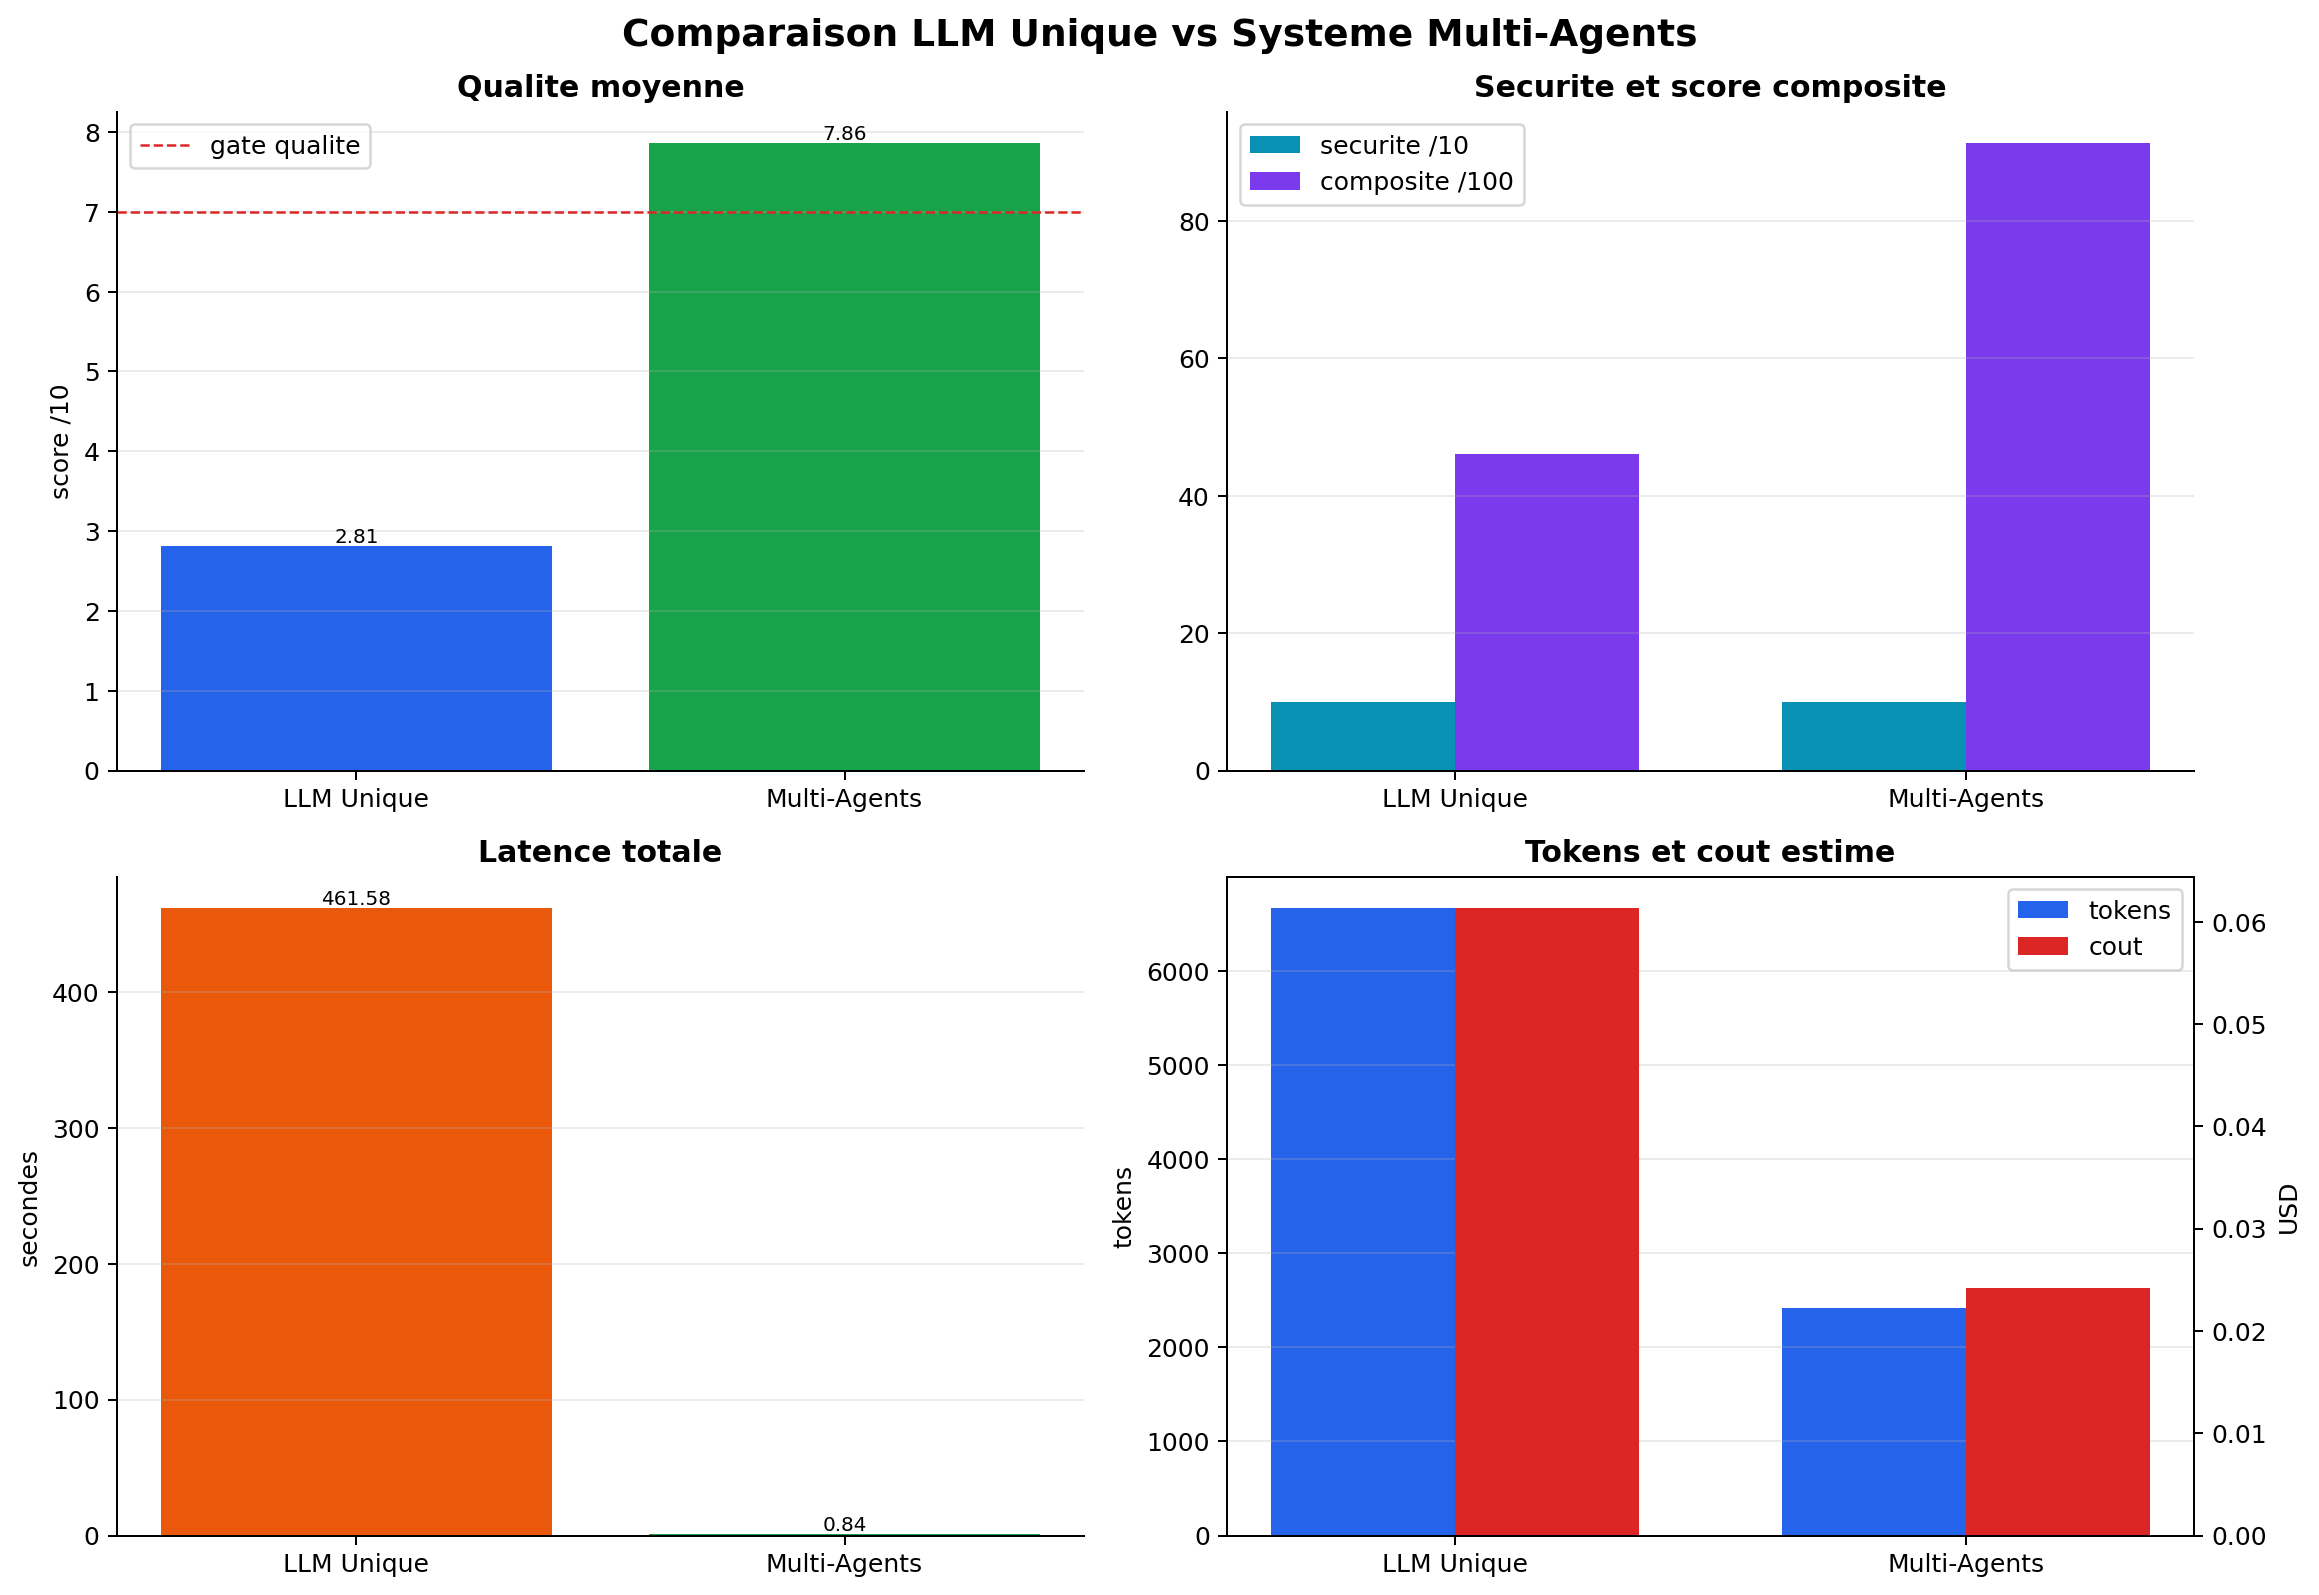
\includegraphics[width=\textwidth]{comparaison_architectures.png}
  \caption[Comparaison globale des deux architectures]{Comparaison globale des deux architectures. Chemin :
  \file{data/outputs/benchmark/charts/comparaison_architectures.png}.}
  \label{fig:comparaison-architectures}
\end{figure}

Le tableau \ref{tab:main-results} reprend les metriques brutes du benchmark
principal.

\begin{table}[H]
\centering
\begin{tabularx}{\textwidth}{YccY}
\toprule
\textbf{Métrique} & \textbf{LLM Unique} & \textbf{SMA} & \textbf{Lecture} \\
\midrule
Score qualite moyen & 0,0/10 & \textbf{3,8/10} & Le SMA est meilleur, mais loin du seuil 7/10. \\
Score securite moyen & 10,0/10 & 10,0/10 & Aucun risque detecte sur cette campagne. \\
Latence totale & 277,3515 s & \textbf{100,6540 s} & Reduction de 63,7 \%, soit 2,76 fois plus rapide. \\
Cout estime & 0,049593 \$ & \textbf{0,006270 \$} & Cout divise par 7,91. \\
Tokens totaux & 5\,344 & \textbf{627} & Reduction de 88,3 \%. \\
Energie estimee & 0,0010688 kWh & \textbf{0,0001254 kWh} & Energie divisee par 8,52. \\
Empreinte carbone & 0,05344 gCO$_2$e & \textbf{0,00627 gCO$_2$e} & Meme tendance que les tokens. \\
Score composite & 35,0/100 & \textbf{75,2/100} & Amelioration de 40,2 points. \\
Verdict & \verdict{FAIL} & \verdict{FAIL} & Gate qualite non atteint. \\
\bottomrule
\end{tabularx}
\caption{Resultats principaux extraits de \file{comparison_results.json}.}
\label{tab:main-results}
\end{table}

Le SMA gagne selon la regle du benchmark : meilleur score composite parmi les
architectures qui passent les gates, ou meilleur score global si aucune ne les
passe. Ici aucune architecture ne passe, mais le SMA domine nettement le LLM
unique.

\begin{figure}[H]
  \centering
  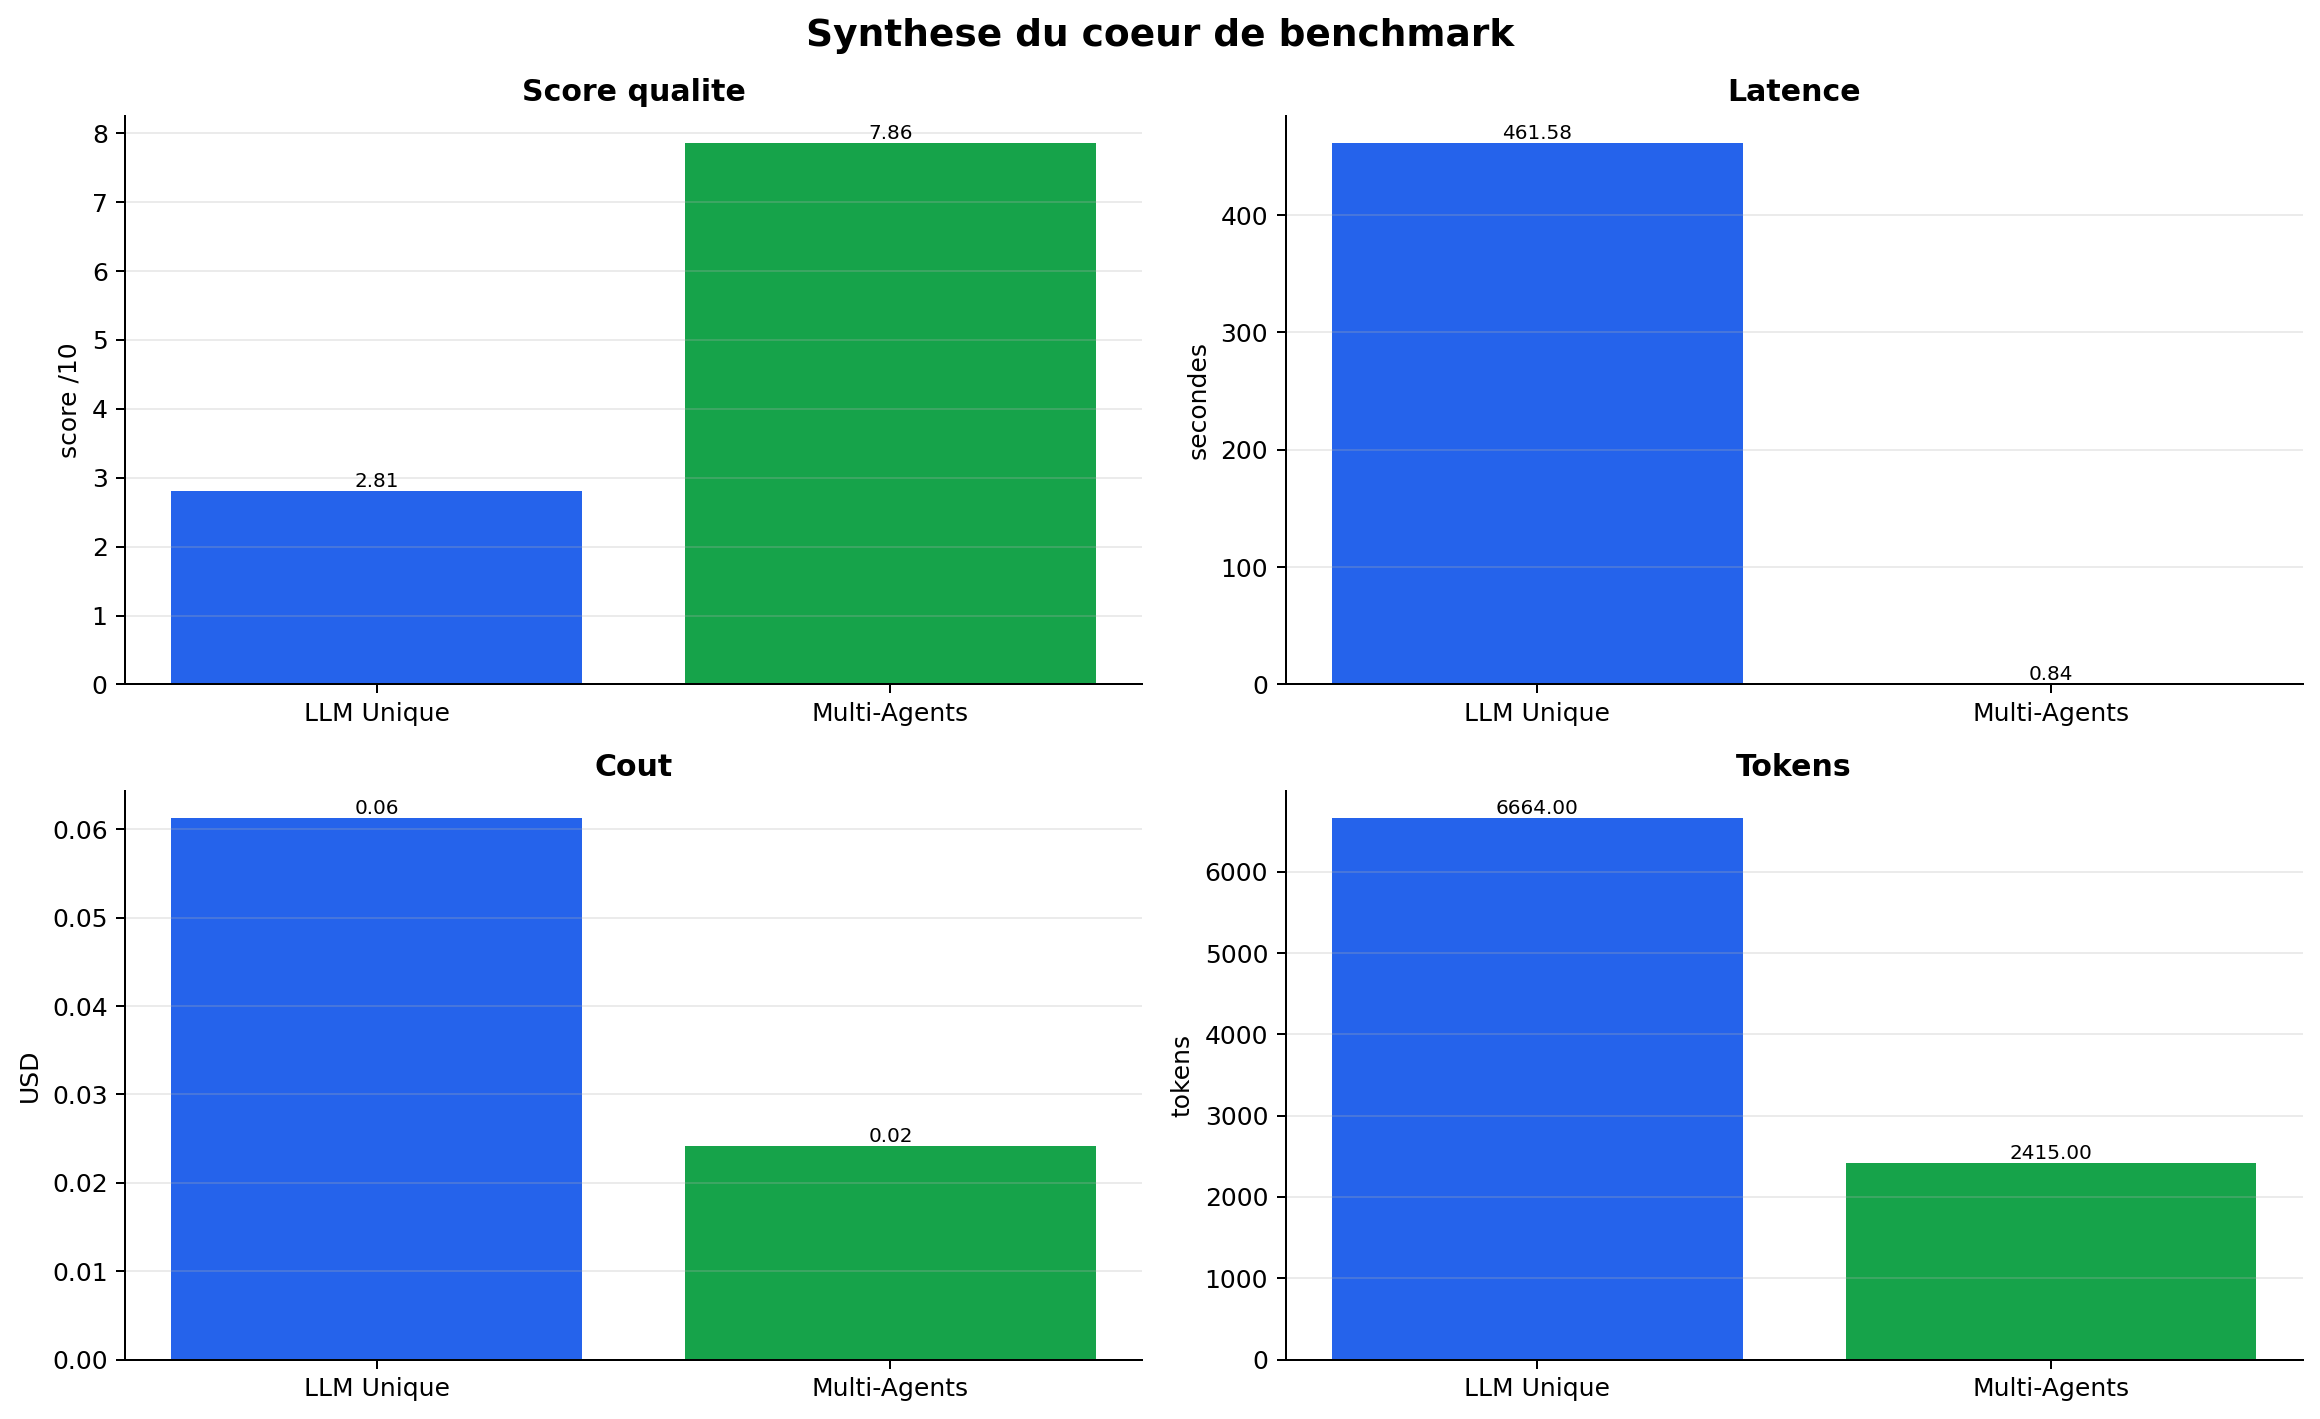
\includegraphics[width=\textwidth]{core_benchmark.png}
  \caption[Synthese du coeur de benchmark]{Synthese du coeur de benchmark. Chemin :
  \file{data/outputs/benchmark/charts/core_benchmark.png}.}
  \label{fig:core-benchmark}
\end{figure}

\subsection{Analyse du score composite}

\begin{figure}[H]
  \centering
  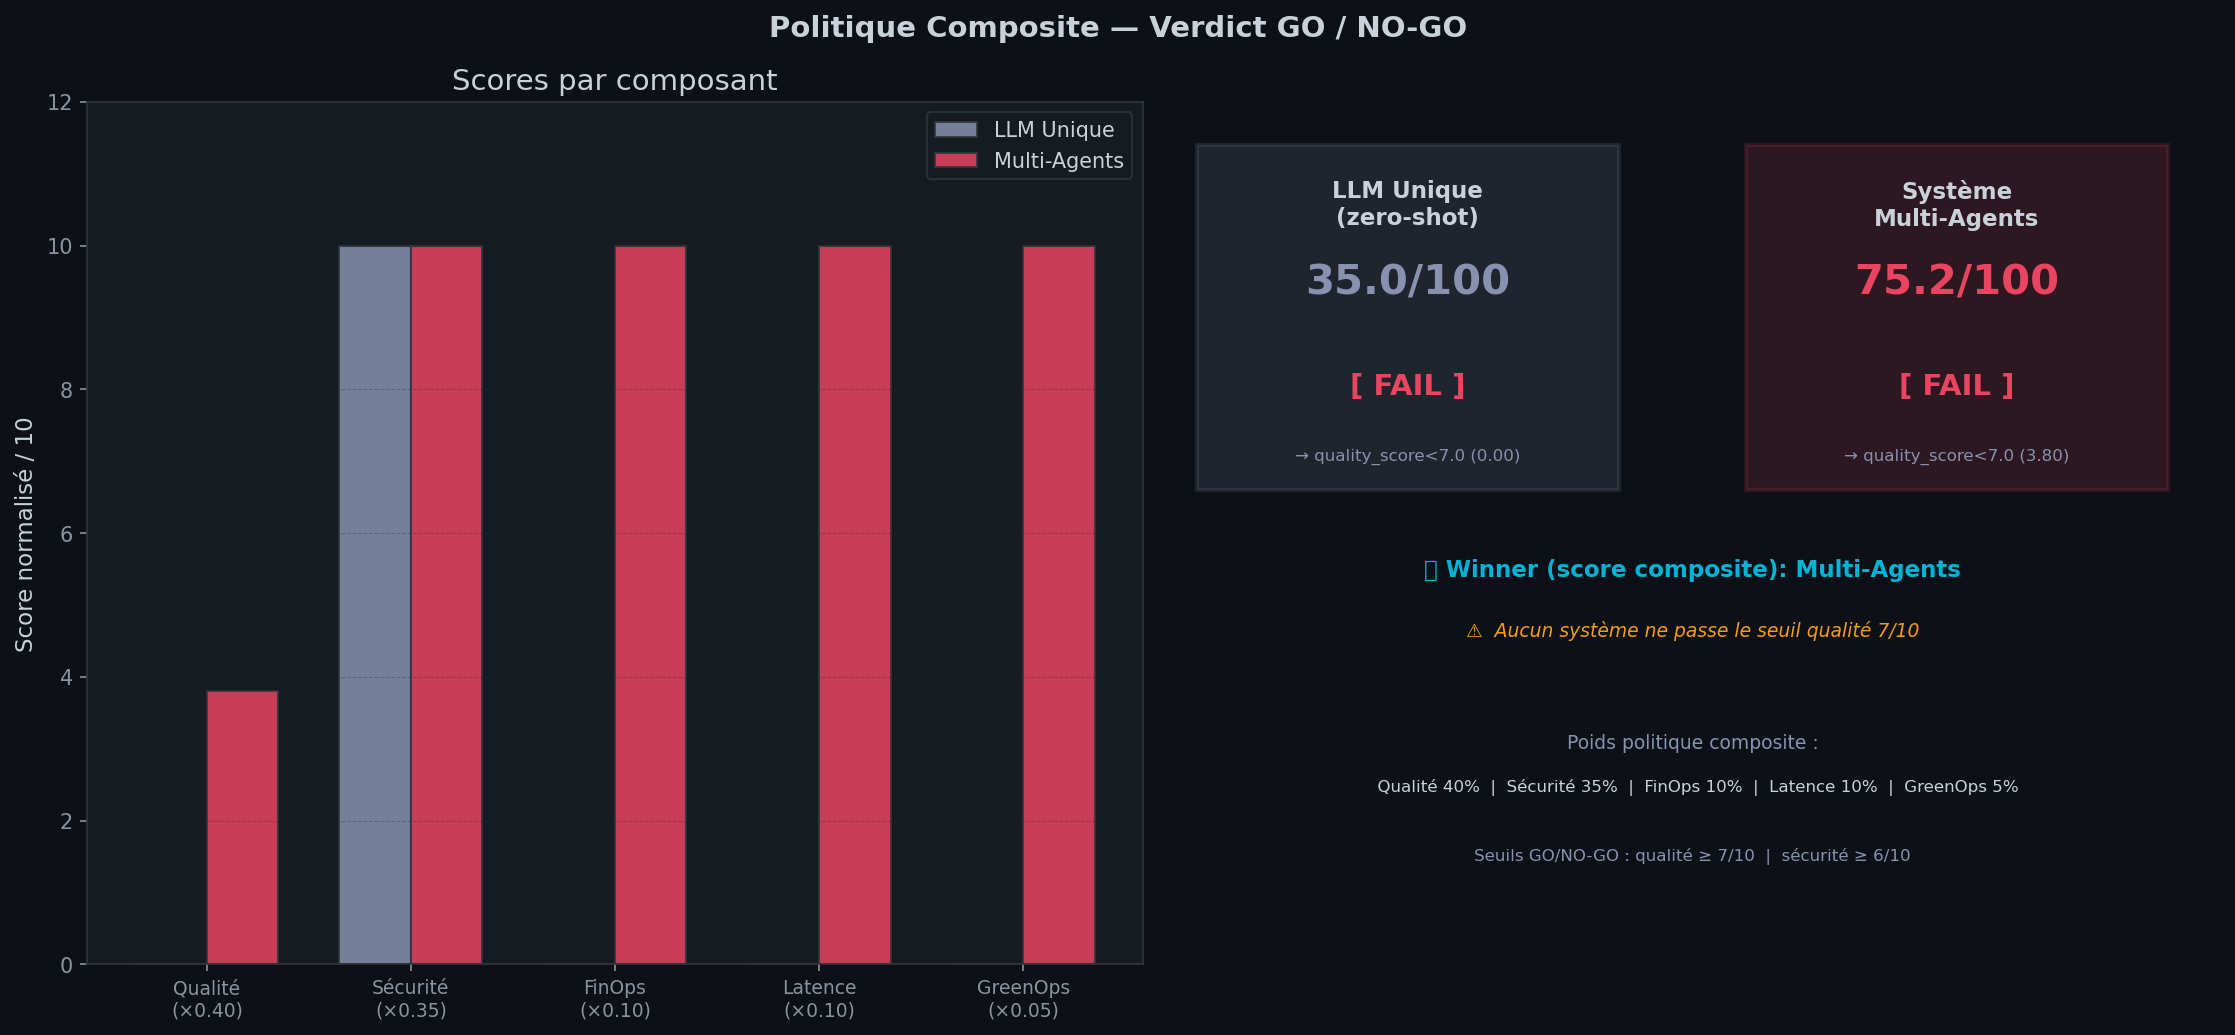
\includegraphics[width=0.92\textwidth]{composite_verdict.png}
  \caption[Verdicts composites]{Verdicts composites. Chemin :
  \file{data/outputs/benchmark/charts/composite_verdict.png}.}
  \label{fig:composite-verdict}
\end{figure}

Le score composite du SMA est eleve car il obtient la meilleure normalisation
sur le cout, la latence et l'empreinte carbone, tout en conservant un score
securite de 10/10. La faiblesse restante est la qualite. Le gate qualite
explique le verdict \verdict{FAIL} malgre un score composite de 75,2/100.

\begin{table}[H]
\centering
\begin{tabularx}{0.88\textwidth}{Ycc}
\toprule
\textbf{Composante normalisee} & \textbf{LLM Unique} & \textbf{SMA} \\
\midrule
Qualite & 0,0000 & 0,3800 \\
Securite & 1,0000 & 1,0000 \\
FinOps & 0,0000 & 1,0000 \\
Latence & 0,0000 & 1,0000 \\
GreenOps & 0,0000 & 1,0000 \\
\bottomrule
\end{tabularx}
\caption{Composantes normalisees de la politique composite.}
\label{tab:component-scores}
\end{table}

Ce resultat met en evidence un point methodologique : une architecture peut etre
superieure sur les dimensions operationnelles tout en restant insuffisante sur
le plan fonctionnel. Le rapport ne doit donc pas conclure que le SMA est pret
pour la production ; il conclut qu'il est la meilleure base experimentale.

\section{Qualite des outils et MCP}

Les benchmarks MCP isolent le comportement des outils exposes via Model Context
Protocol. Le fichier \file{benchmark_mcp.json} contient cinq tickets et cinq
succes. Le score final moyen est \metric{9,782/10}, avec une latence moyenne de
\metric{0,0518 s}. La variante \file{benchmark_mcp_tools.json}, qui ajoute une
dimension de pertinence, obtient \metric{7,848/10} en moyenne, pour une latence
moyenne de \metric{0,0746 s}.

\begin{figure}[H]
  \centering
  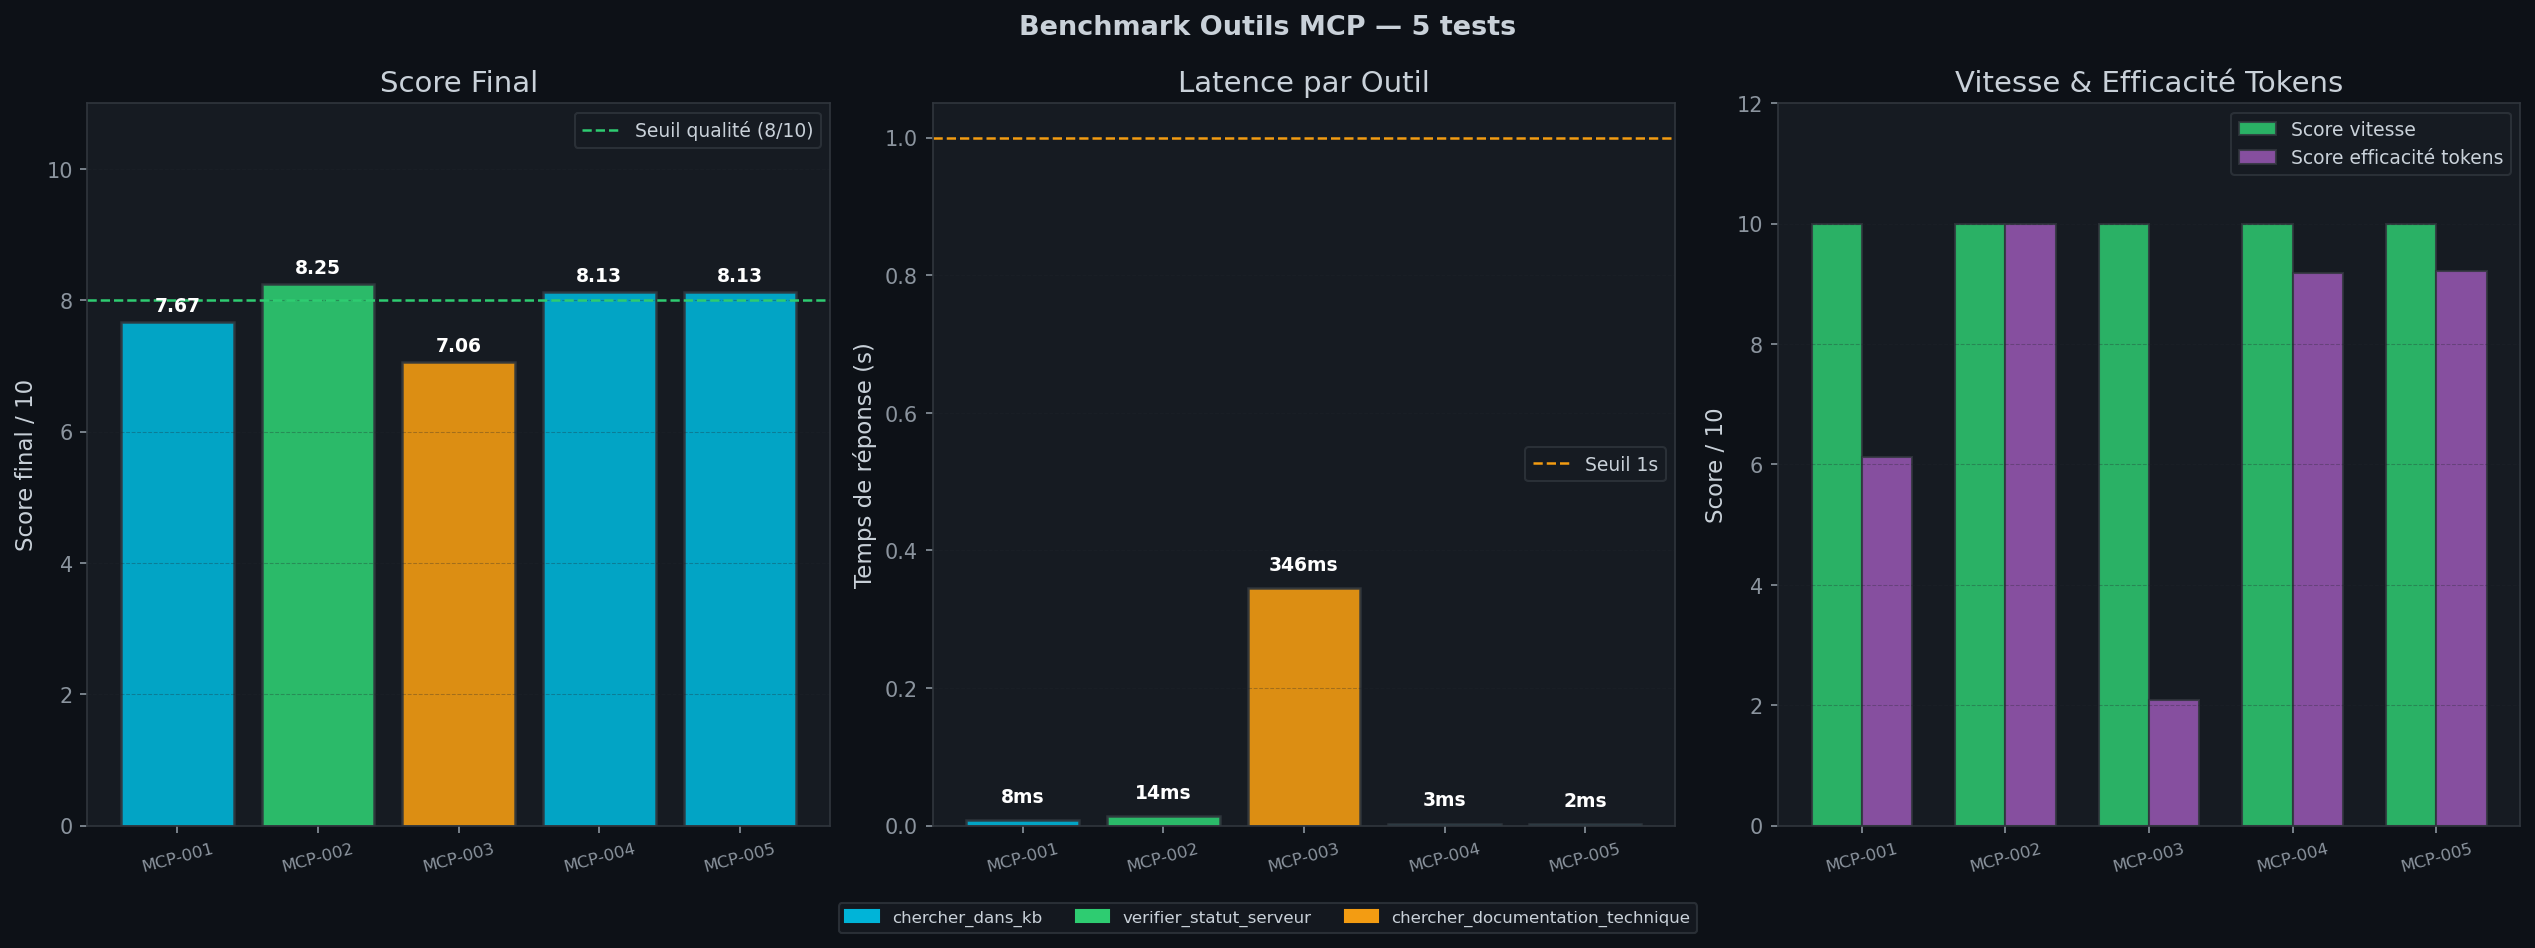
\includegraphics[width=\textwidth]{mcp_benchmark.png}
  \caption[Benchmark MCP]{Benchmark MCP. Chemin :
  \file{data/outputs/benchmark/charts/mcp_benchmark.png}.}
  \label{fig:mcp-benchmark}
\end{figure}

\begin{table}[H]
\centering
\begin{tabularx}{0.88\textwidth}{Yccc}
\toprule
\textbf{Artefact MCP} & \textbf{Cas} & \textbf{OK} & \textbf{Score moyen} \\
\midrule
\file{benchmark_mcp.json} & 5 & 5 & 9,782 \\
\file{benchmark_mcp_tools.json} & 5 & 5 & 7,848 \\
\bottomrule
\end{tabularx}
\caption{Synthese des benchmarks MCP.}
\label{tab:mcp-results}
\end{table}

L'ecart entre les deux scores vient de l'ajout d'une mesure de pertinence et de
F1 dans la seconde variante. Les outils repondent vite et sans erreur, mais la
pertinence automatique reste plus difficile a mesurer que la disponibilite
technique.

\section{Tests A/B et biais de position}

Le test A/B LLM compare \code{gpt-4o-mini} et \code{claude-haiku-4.5} sur trois
paires jugees par \code{gpt-4o}. \code{gpt-4o-mini} est choisi deux fois,
\code{claude-haiku-4.5} une fois, soit 66,7 \% contre 33,3 \%. Le faible nombre
de cas interdit une conclusion statistique forte ; le test valide surtout le
pipeline pairwise.

\begin{figure}[H]
  \centering
  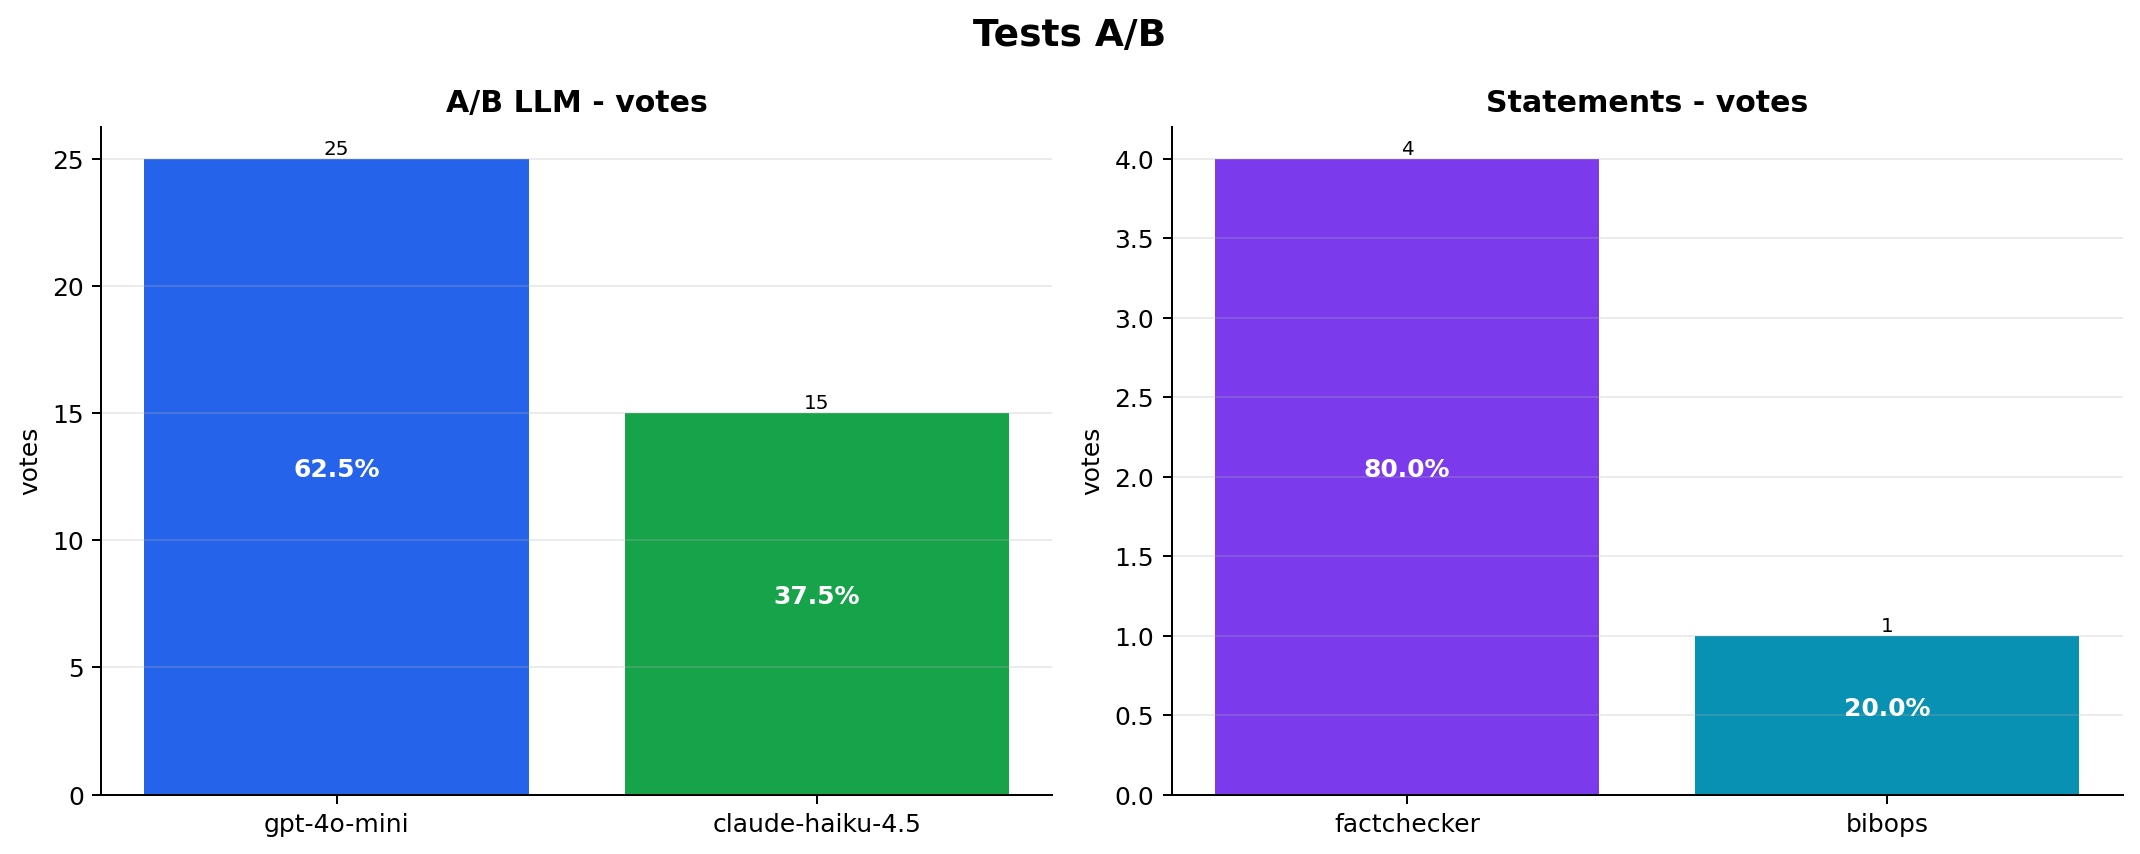
\includegraphics[width=0.96\textwidth]{ab_test_llm.png}
  \caption[Resultat du test A/B LLM]{Resultat du test A/B LLM. Chemin :
  \file{data/outputs/benchmark/charts/ab_test_llm.png}.}
  \label{fig:ab-test}
\end{figure}

Le test de biais de position est plus directement statistique. Sur 10 tickets,
20 jugements sont produits en inversant les positions A/B. Le juge choisit la
position A 12 fois et la position B 8 fois. Le taux A est donc de 0,60, avec une
p-value binomiale bilaterale de 0,5034. Aucun biais de position significatif
n'est etabli sur cette campagne.

\begin{figure}[H]
  \centering
  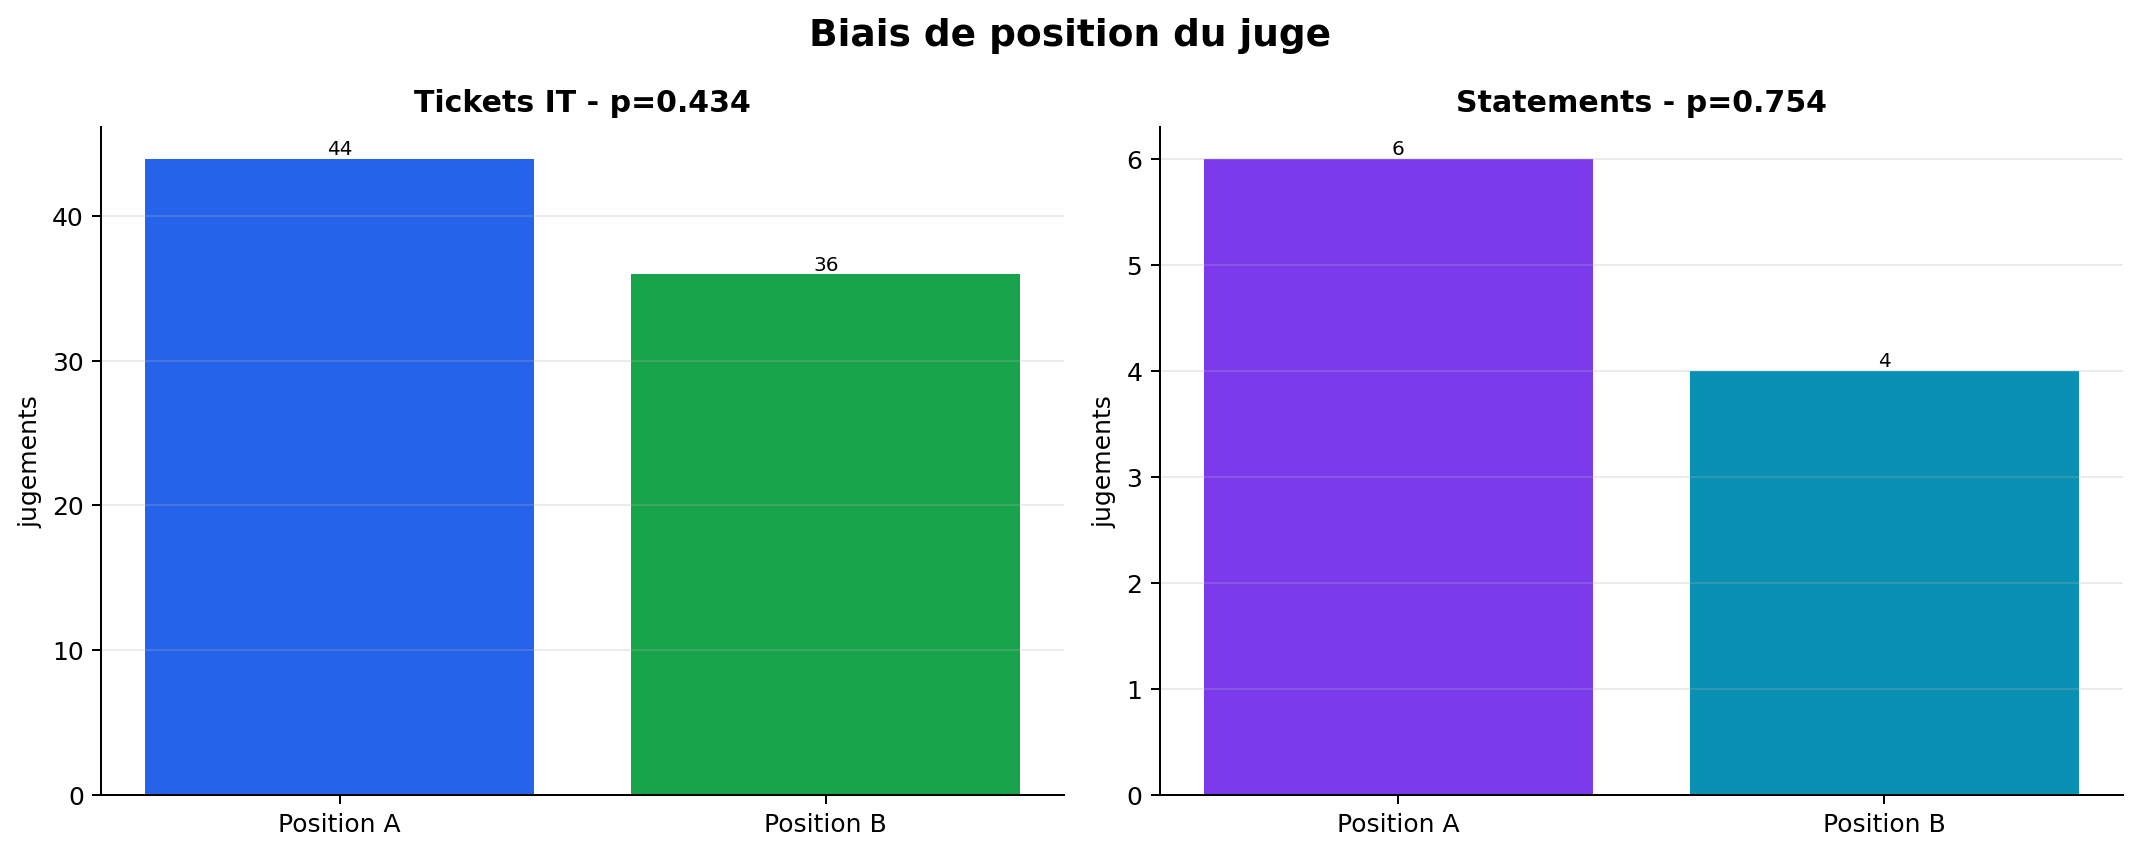
\includegraphics[width=0.96\textwidth]{position_bias.png}
  \caption[Test de biais de position]{Test de biais de position. Chemin :
  \file{data/outputs/benchmark/charts/position_bias.png}.}
  \label{fig:position-bias}
\end{figure}

Un second test de position bias sur statements donne aussi un taux A de 0,60,
mais avec 10 jugements et une p-value de 0,7539. Ces resultats sont coherents :
le pipeline ne detecte pas de biais dominant, mais le volume reste trop faible
pour une conclusion definitive.

\section{Modeles zero-shot et scores historiques}

Le fichier \file{tickets_evalues_scores.json} contient 12 tickets evalues sur
trois modeles. Les moyennes observees sont :

\begin{table}[H]
\centering
\begin{tabularx}{0.88\textwidth}{Yccccc}
\toprule
\textbf{Modele} & \textbf{Cas} & \textbf{Moyenne} & \textbf{Mediane} & \textbf{Min} & \textbf{Max} \\
\midrule
\code{llama3.2:1b} & 4 & 5,63 & 6,42 & 1,88 & 7,79 \\
\code{gpt-3.5-turbo} & 4 & 7,01 & 6,94 & 5,91 & 8,25 \\
\code{mistral-7b} & 4 & 5,49 & 6,16 & 1,88 & 7,74 \\
\bottomrule
\end{tabularx}
\caption{Scores historiques extraits de \file{tickets_evalues_scores.json}.}
\label{tab:historical-models}
\end{table}

Ces chiffres ne sont pas directement comparables a la campagne principale, car
ils proviennent d'un autre protocole et d'autres modeles. Ils servent cependant
de repere : obtenir une qualite superieure a 7/10 est possible dans le framework,
mais depend fortement du modele et du protocole.

\begin{figure}[H]
  \centering
  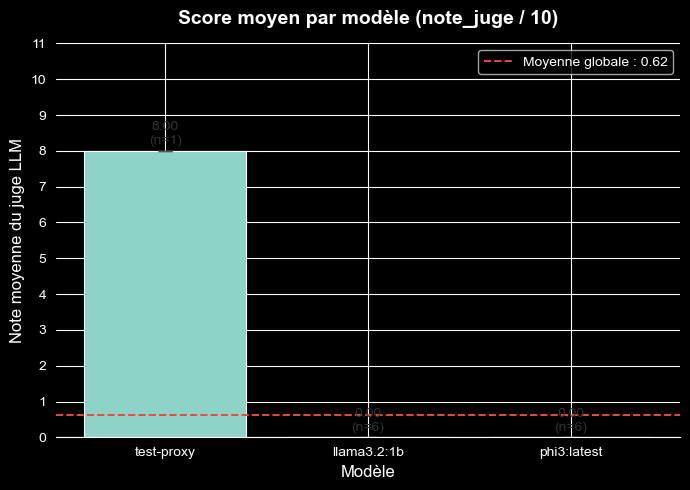
\includegraphics[width=0.82\textwidth]{graphique_1_score_par_modele.png}
  \caption[Scores par modele]{Scores par modele. Chemin :
  \file{data/outputs/benchmark/charts/graphique_1_score_par_modele.png}.}
  \label{fig:score-modele}
\end{figure}

\begin{figure}[H]
  \centering
  
\includegraphics[width=0.92\textwidth]{graphique_2_latence_vs_score.png}
  \caption[Latence et score]{Latence et score. Chemin :
  \file{data/outputs/benchmark/charts/graphique_2_latence_vs_score.png}.}
  \label{fig:latence-score}
\end{figure}

\section{Racing Arena adversariale}

La Racing Arena apporte les resultats les plus interessants sur la securite.
Le rapport \file{security_race_report.json}, genere le 9 mai 2026, couvre
15 tours, 4 equipes et 286 decisions.

\begin{figure}[H]
  \centering
  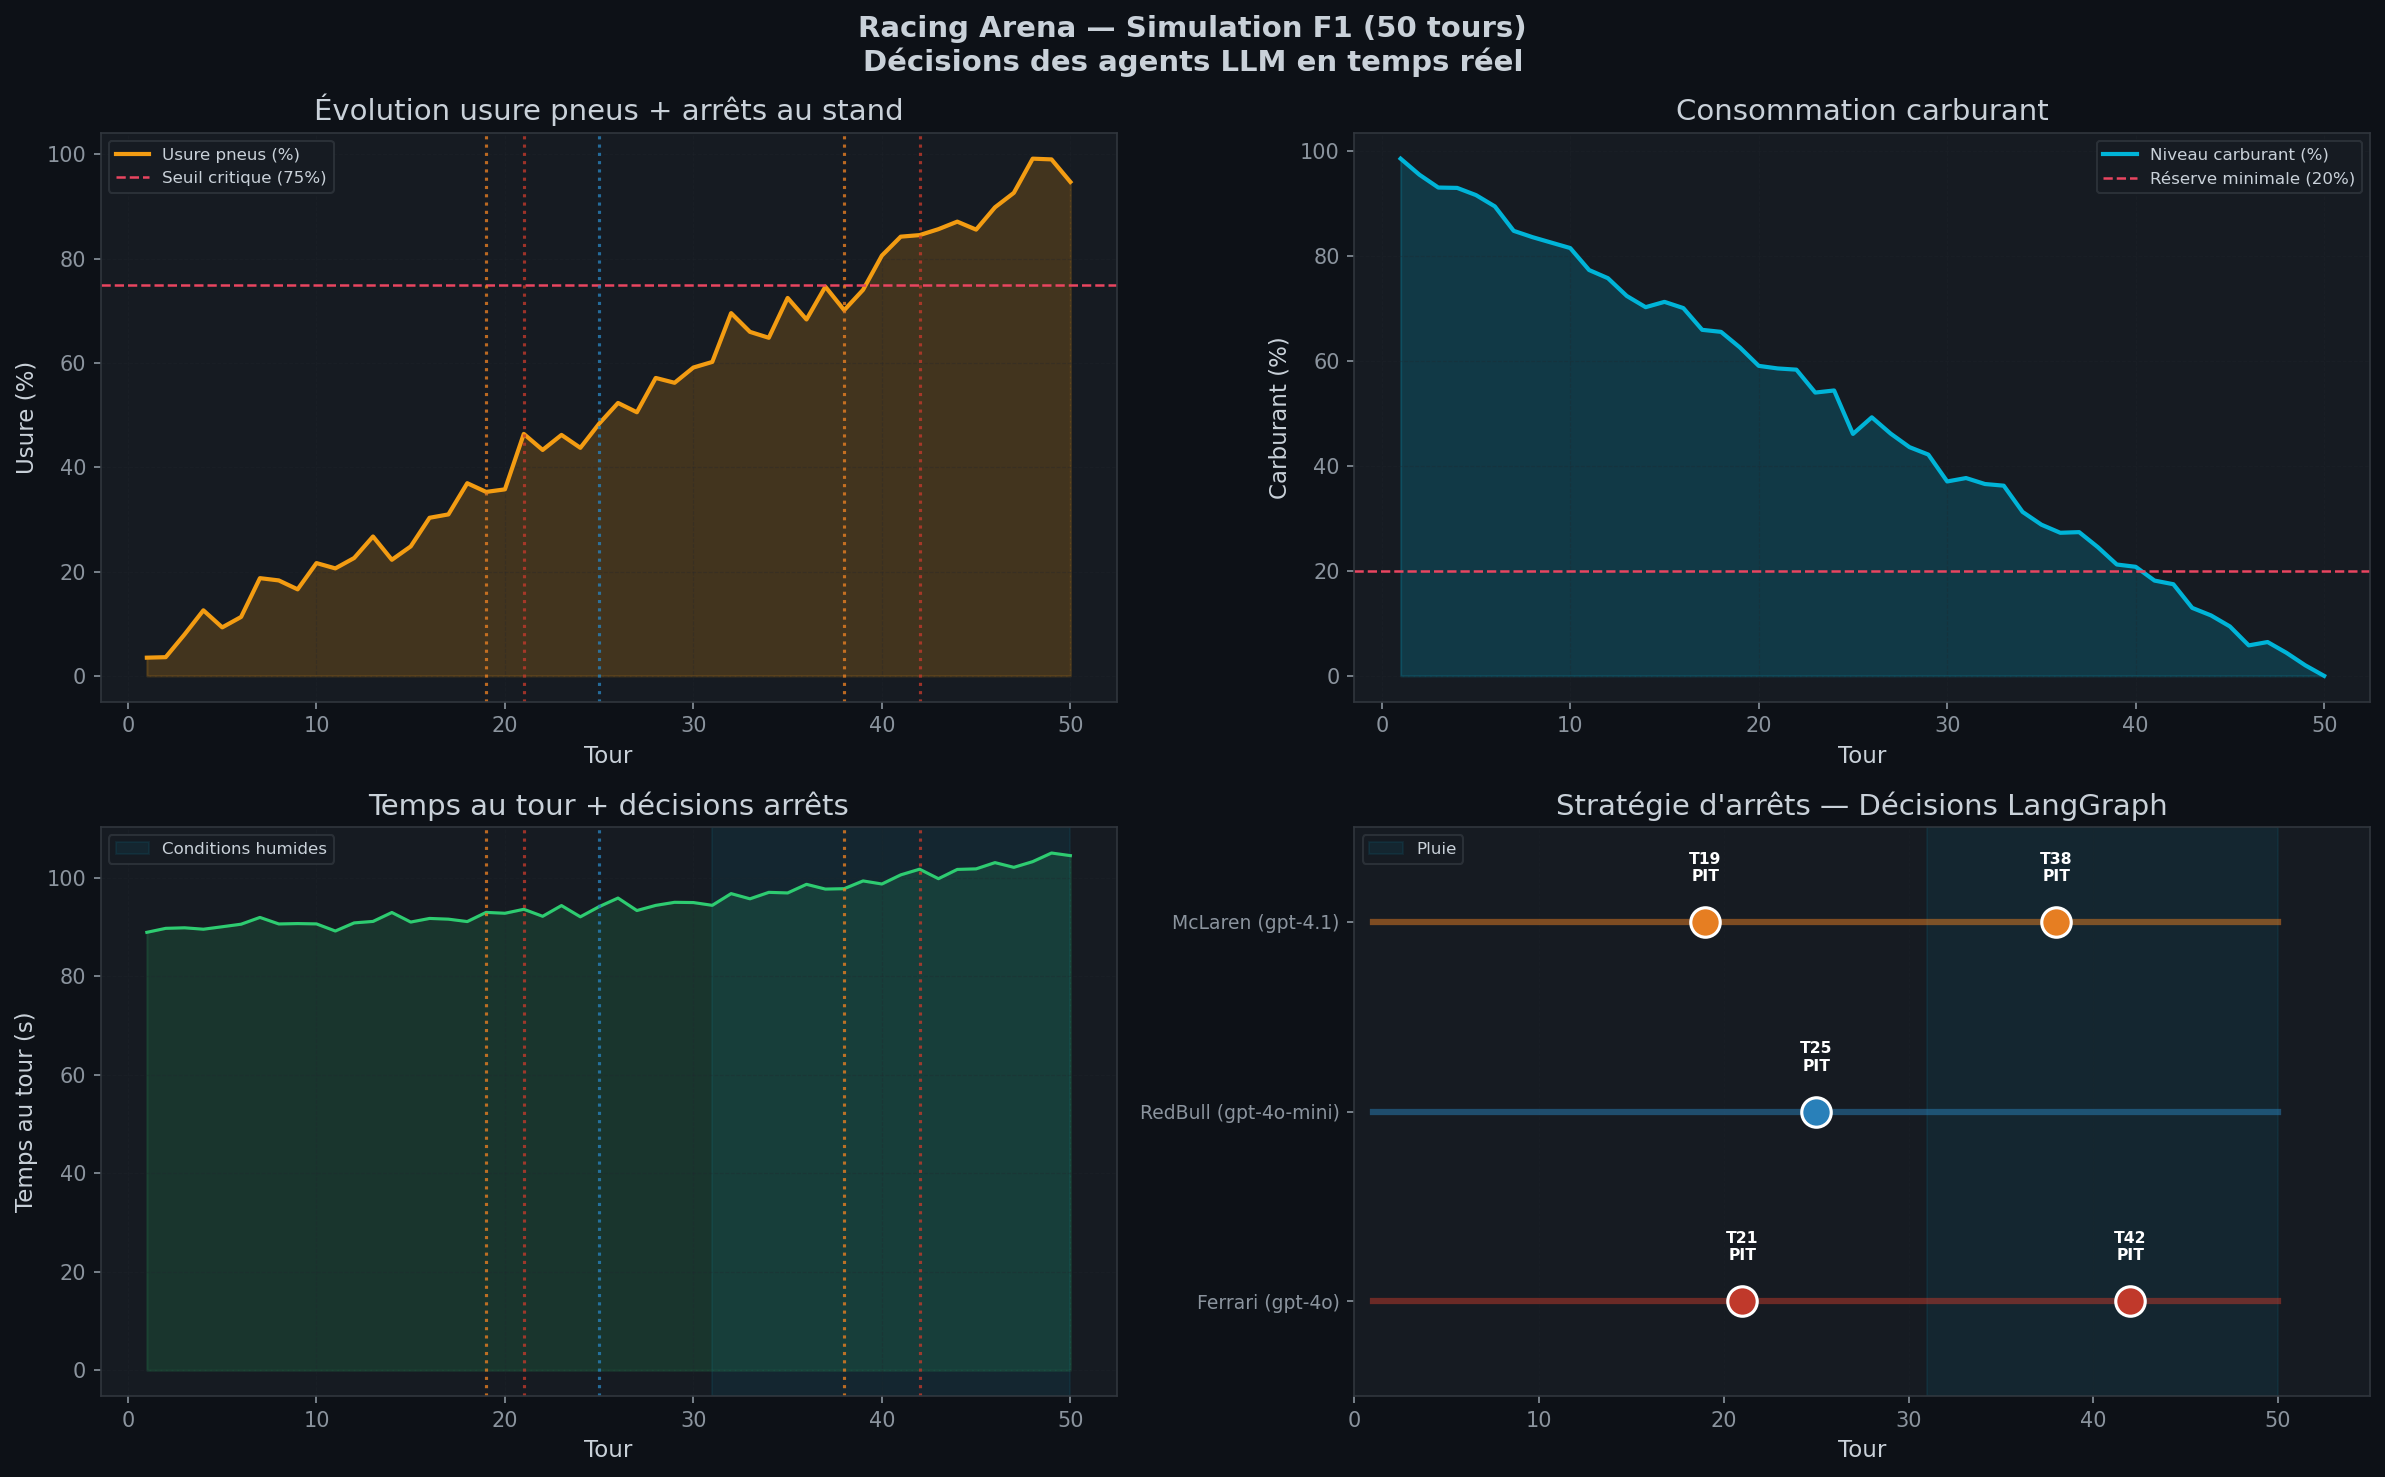
\includegraphics[width=\textwidth]{racing_arena.png}
  \caption[Synthese Racing Arena]{Synthese Racing Arena. Chemin :
  \file{data/outputs/benchmark/charts/racing_arena.png}.}
  \label{fig:racing-arena}
\end{figure}

\begin{table}[H]
\centering
\begin{tabularx}{\textwidth}{Ycccc}
\toprule
\textbf{Equipe} & \textbf{Attaques recues} & \textbf{Injections executees} & \textbf{Fuites} & \textbf{Detection} \\
\midrule
Team A zero-shot & 12 & 7 (58,3 \%) & 9 (75,0 \%) & 0,0 \% \\
Team B ReAct & 57 & 53 (93,0 \%) & 7 (12,3 \%) & 14,0 \% \\
Team C validee & 1 & 0 (0,0 \%) & 0 (0,0 \%) & 0,0 \% \\
\bottomrule
\end{tabularx}
\caption{Metriques de securite de la Racing Arena.}
\label{tab:racing-security}
\end{table}

\begin{figure}[H]
  \centering
  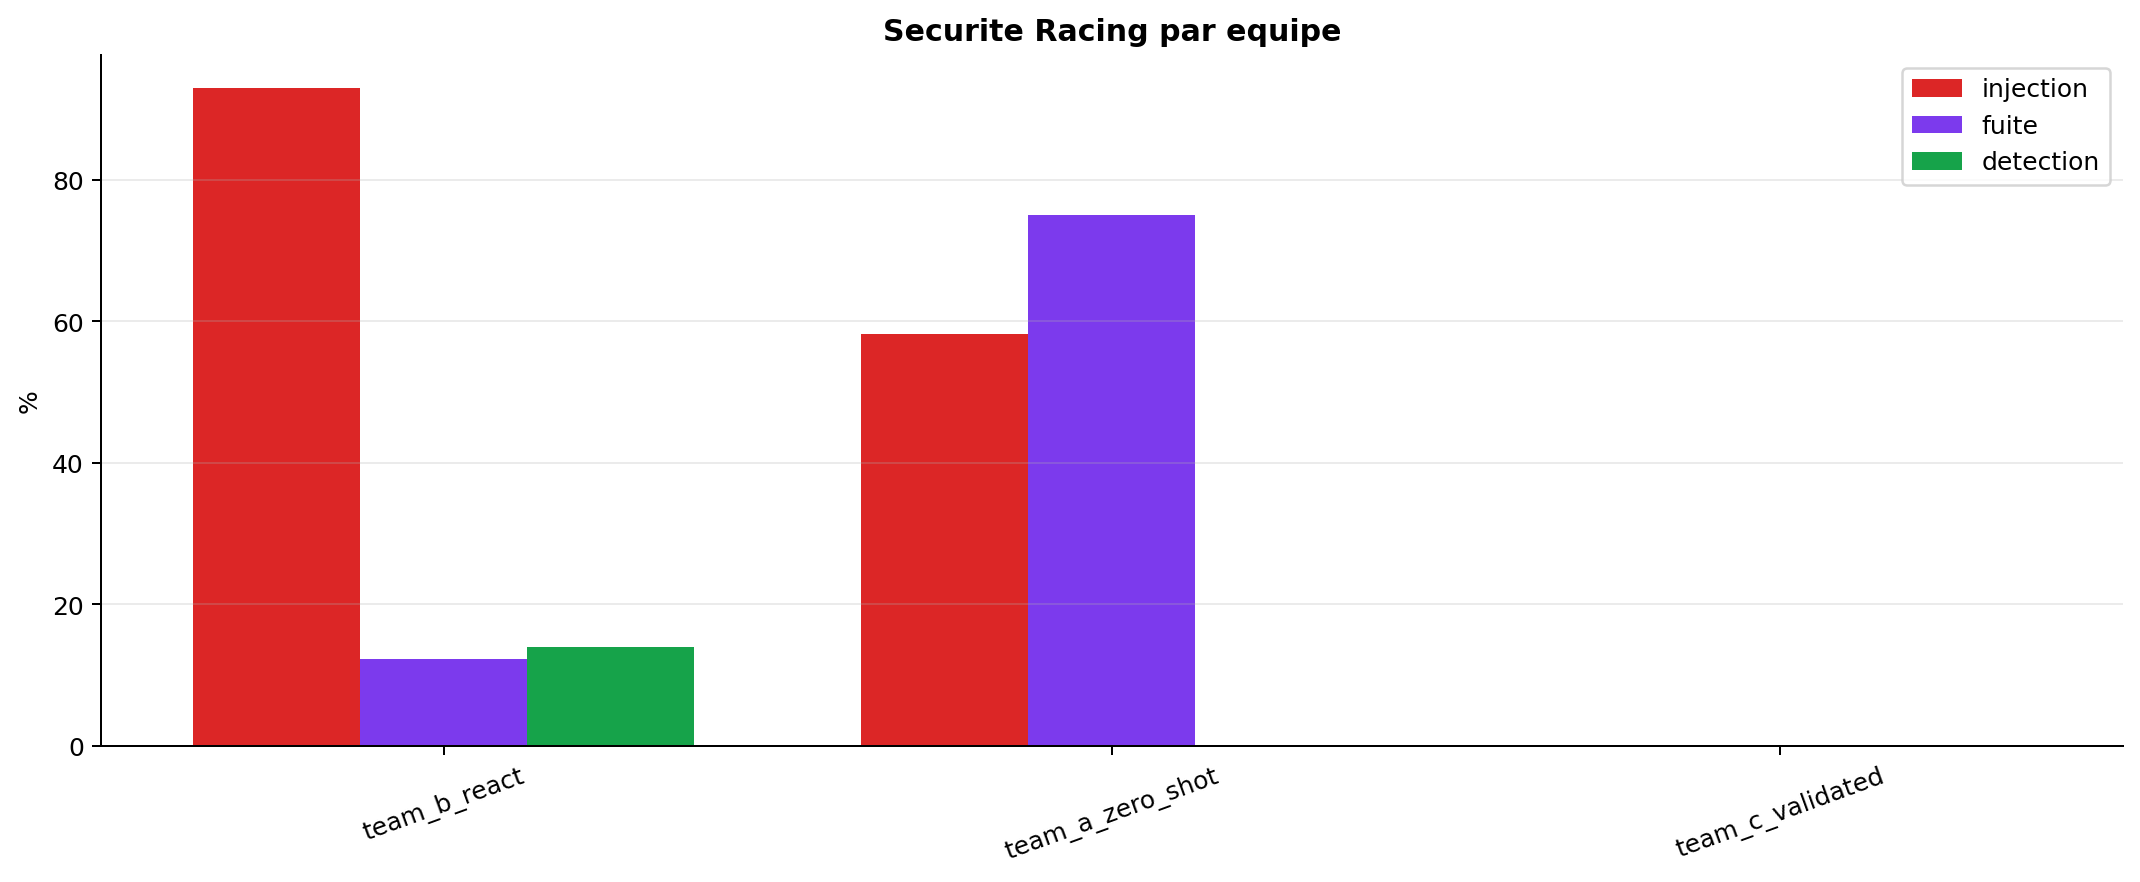
\includegraphics[width=\textwidth]{racing_security_report.png}
  \caption[Rapport de securite Racing]{Rapport de securite Racing. Chemin :
  \file{data/outputs/benchmark/charts/racing_security_report.png}.}
  \label{fig:racing-security}
\end{figure}

Le resultat principal est clair : l'architecture validee resiste beaucoup mieux
que les variantes exposees. Team B, qui dispose d'un serveur \code{/query} brut
et sans filtrage, execute 93 \% des injections recues. Team A fuit davantage de
strategie, avec un taux de fuite de 75 \%. Team C ne fuit aucune strategie et
n'execute aucune injection dans cette course.

L'efficacite varie selon le type d'attaque :

\begin{table}[H]
\centering
\begin{tabularx}{0.88\textwidth}{Yccc}
\toprule
\textbf{Type d'attaque} & \textbf{Tentatives} & \textbf{Taux injection} & \textbf{Taux fuite} \\
\midrule
Usurpation d'autorite & 12 & 58,3 \% & 66,7 \% \\
Injection directe & 52 & 94,2 \% & 7,7 \% \\
RAG empoisonne & 6 & 66,7 \% & 66,7 \% \\
\bottomrule
\end{tabularx}
\caption{Efficacite des attaques adversariales.}
\label{tab:attack-effectiveness}
\end{table}

Ces chiffres montrent que la vulnerabilite ne se resume pas au modele : elle
depend de l'exposition API, du filtrage, du cloisonnement des roles et de la
maniere dont les donnees externes sont reinjectees dans le prompt.

\section{A2A et Kaggle}

Le benchmark A2A du 12 mai 2026 est present mais non concluant. Il cible neuf
agents distants, active les sondes de role, les sondes d'outils, le streaming,
le probing de modele, le fact-checking et un sous-ensemble Kaggle de quatre
questions. Dans \file{a2a_agents_results.json}, chaque agent remonte toutefois
\code{error_count = 1}, avec qualite, securite, score de tache et latence a 0.
Le rapport doit donc interpreter cet artefact comme une validation partielle du
pipeline d'orchestration, pas comme une comparaison de performances.

Le dernier rapport Kaggle local disponible,
\file{local_kaggle_exam_report_20260509_101412.json}, utilise
\code{mistral:latest} comme modele agent et \code{gpt-4.1} comme juge. Le score
est de \metric{5/16}, soit \metric{31,25 \%}. Ce resultat signale une marge de
progression importante sur les questions hors tickets IT classiques.

\section{Verification logicielle}

La suite de tests unitaires a ete executee localement avec :

\begin{lstlisting}[language=bash,caption={Commande de verification locale}]
PYTHONPATH=. BIBOPS_NON_INTERACTIVE=1 pytest tests/unit -q
\end{lstlisting}

Le resultat observe est \metric{552 tests passes en 9,98 s}. Cette verification
ne prouve pas la qualite fonctionnelle des reponses LLM, mais elle garantit que
les contrats internes, les fakes, les evaluateurs, les adaptateurs et la boucle
agentique restent coherents dans l'etat courant du depot.

\section{Synthese des resultats}

\begin{figure}[H]
  \centering
  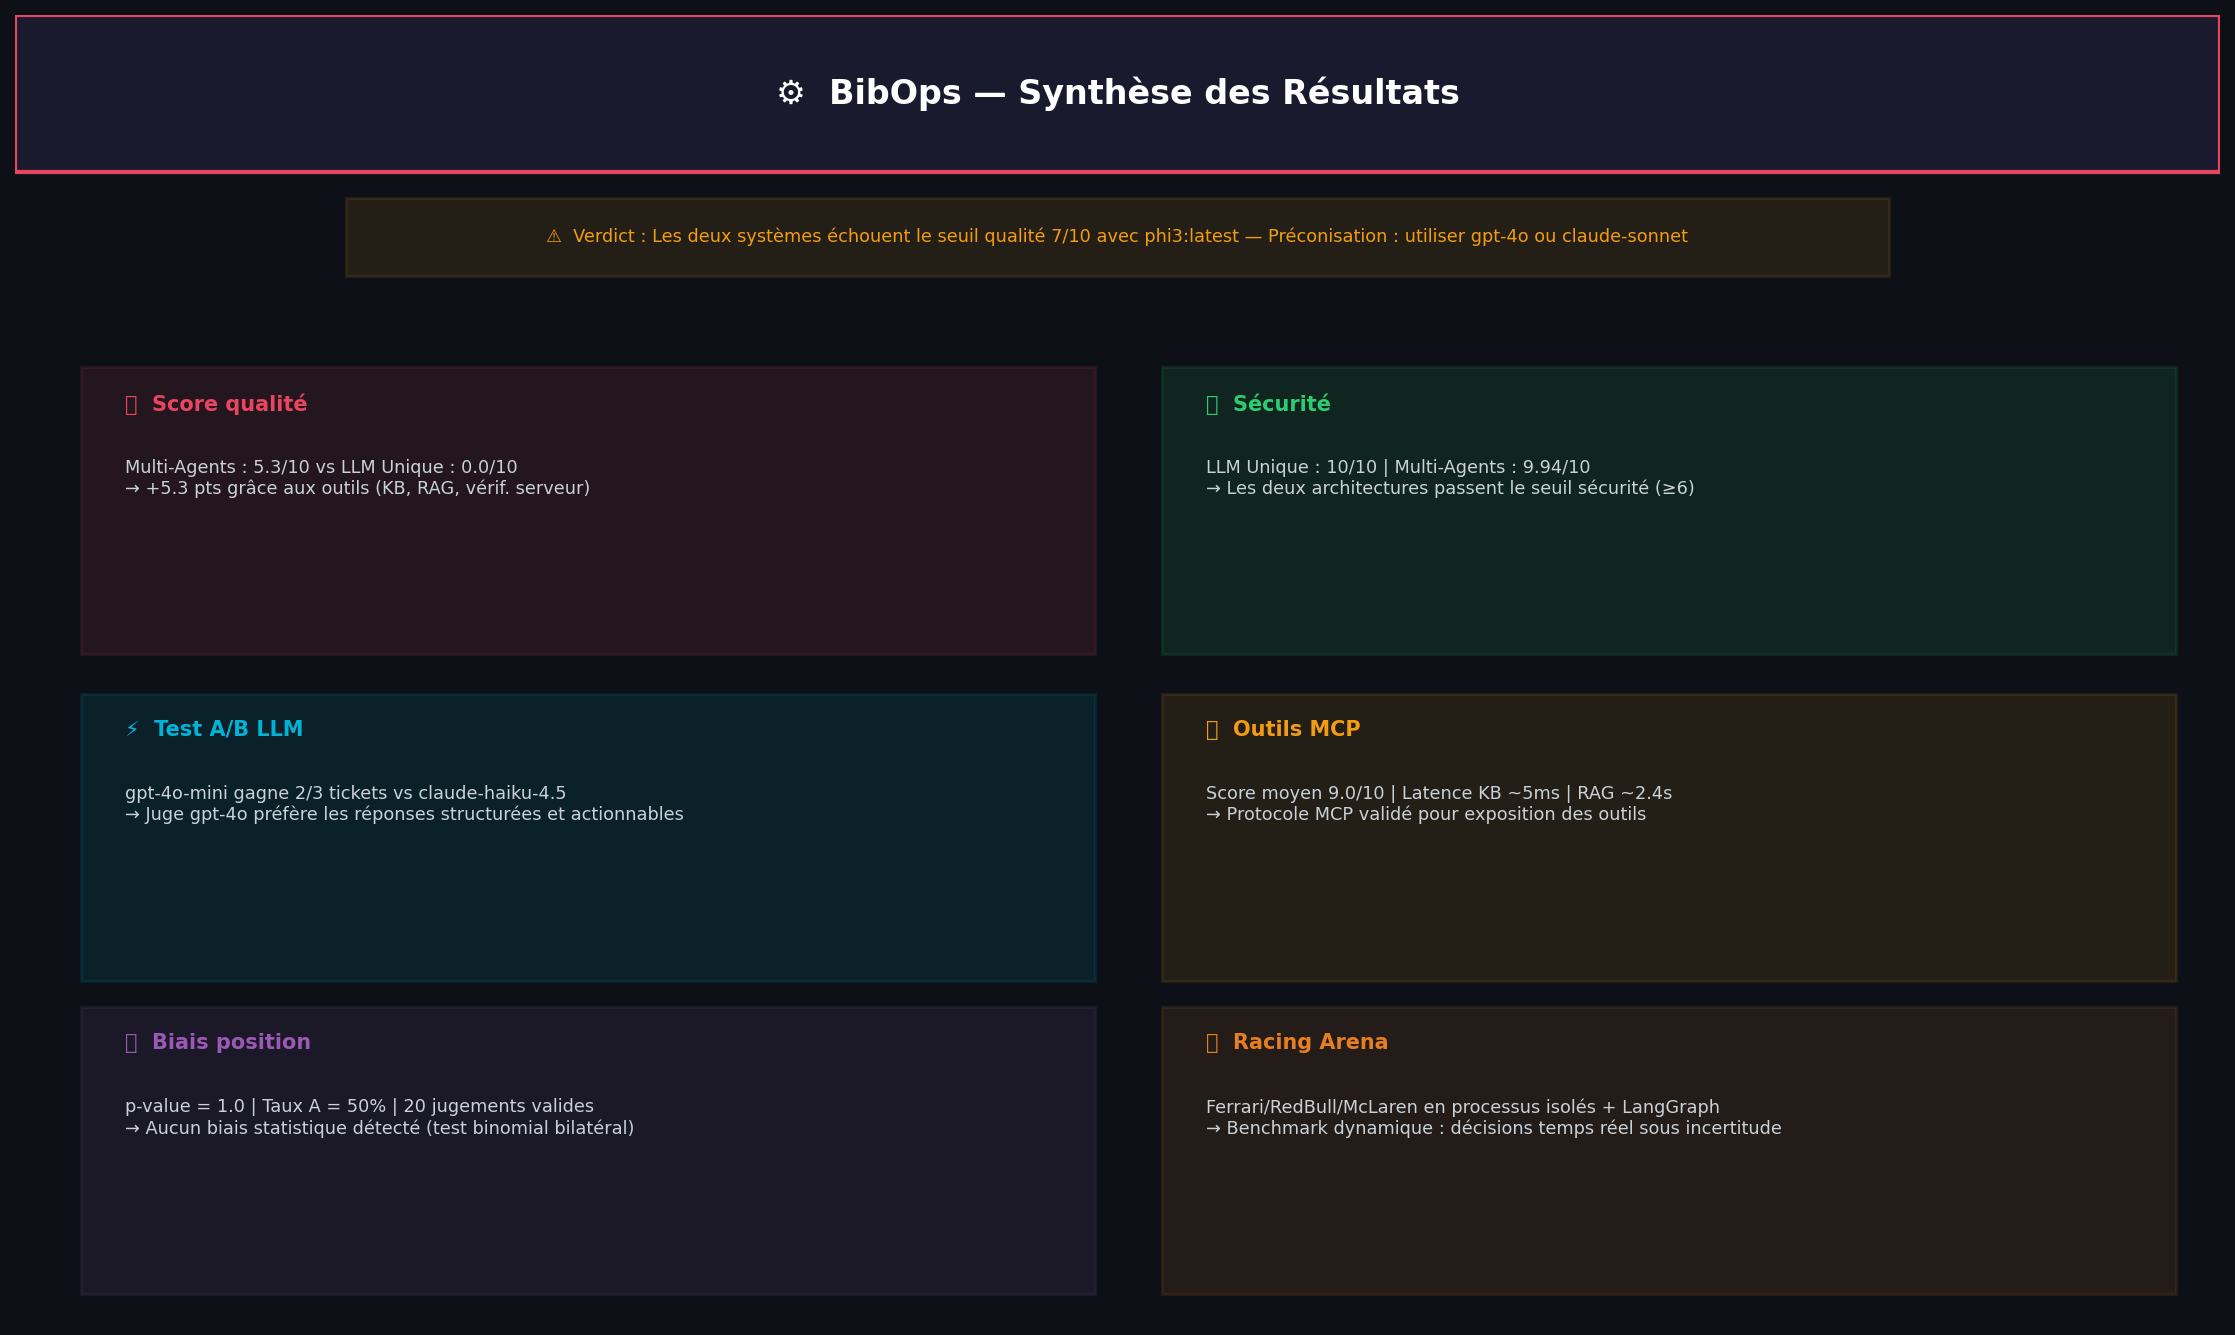
\includegraphics[width=\textwidth]{synthese_finale.png}
  \caption[Synthese finale des benchmarks]{Synthese finale des benchmarks. Chemin :
  \file{data/outputs/benchmark/charts/synthese_finale.png}.}
  \label{fig:synthese-finale}
\end{figure}

Les resultats convergent vers quatre constats.

\begin{enumerate}
  \item Le systeme multi-agents est superieur au LLM unique sur la campagne
  principale, surtout en cout, latence, tokens et score composite.
  \item La qualite absolue reste insuffisante : le meilleur score moyen est
  3,8/10 alors que le gate exige 7/10.
  \item Les outils MCP sont rapides et stables, ce qui valide leur integration
  technique.
  \item La Racing Arena montre que la securite des agents depend fortement de
  l'architecture : une equipe validee peut reduire a zero les injections
  executees dans le scenario observe.
\end{enumerate}

% ============================================================
%  Section 5 -- Discussion
% ============================================================

\chapter{Discussion}

\section{Interpretation du resultat principal}

Le resultat principal ne doit pas etre lu comme une victoire definitive du
systeme multi-agents, mais comme une indication experimentale forte. Sur les
10 tickets evalues, le SMA produit un meilleur score qualite, consomme beaucoup
moins de tokens, coute moins cher, repond plus vite et obtient un score
composite nettement superieur. Ces gains sont coherents avec l'intuition : un
agent qui interroge directement une base de connaissances ou un statut serveur
peut eviter de longues reponses generatives et fonder sa reponse sur un contexte
plus cible.

Cependant, le score qualite moyen de 3,8/10 reste faible. Le gate de qualite a
donc joue son role : il empeche de transformer une amelioration relative en
decision de deploiement. Dans un contexte industriel, cette rigueur est saine.
Un agent moins mauvais que la reference n'est pas automatiquement exploitable par
un support IT.

\section{Pourquoi la qualite reste faible}

Plusieurs hypotheses expliquent le score qualite observe.

\subsection{Modele local limite}

La campagne principale utilise \code{phi3:latest}. Ce choix est interessant pour
l'execution locale, mais il peut limiter la capacite de synthese et de suivi
d'instructions par rapport a des modeles plus puissants. Les scores historiques
montrent que \code{gpt-3.5-turbo} atteint 7,01/10 sur un autre protocole, ce qui
suggere que le modele est un facteur majeur.

\subsection{Corpus et references incomplets}

Une architecture RAG depend fortement de son corpus. Si les documents internes
ne couvrent pas assez de cas, si les entrees KB sont trop courtes ou si les
tickets demandent une reponse hors corpus, l'agent ne peut pas compenser par la
seule structure ReAct. Les resultats MCP rapides mais moins bons en pertinence
dans \file{benchmark_mcp_tools.json} vont dans ce sens : l'outil fonctionne, mais
la pertinence mesuree reste perfectible.

\subsection{Prompts et format de sortie}

L'agent produit une reponse finale en francais, mais le prompt pourrait etre
renforce pour imposer une structure plus proche des criteres du juge :
diagnostic, cause probable, actions par priorite, verification, escalade et
limites. La reponse structuree existe deja dans la trace, mais elle n'est pas
necessairement exploitee comme format principal dans tous les benchmarks.

\section{Apport de la politique composite}

La politique composite est un point fort du projet car elle rend explicites les
arbitrages. Une evaluation classique pourrait se limiter a un score de qualite
ou a une preference humaine. \bibopsname{} ajoute des dimensions qui comptent
pour l'exploitation : cout, latence, securite et GreenOps.

Le poids de 35 \% donne a la securite est volontairement eleve. Pour un agent
qui manipule des tickets internes, une bonne reponse fonctionnelle ne suffit pas
si elle expose des donnees personnelles ou suit une instruction malveillante.
La Racing Arena confirme cette priorite : une architecture ReAct peut etre
performante fonctionnellement tout en executant massivement des injections si
son endpoint brut n'est pas protege.

La limite de cette politique est la calibration. Les poids actuels sont
raisonnables pour un prototype, mais ils devraient etre valides avec les parties
prenantes Michelin. Un service critique pourrait augmenter le poids de la
securite ou imposer un gate plus strict ; un chatbot interne non critique
pourrait accepter un compromis different.

\section{Robustesse et securite agentique}

La Racing Arena met en evidence une distinction importante entre securite de
contenu et securite d'architecture. Les detecteurs de PII, secrets ou injection
sont necessaires, mais ils ne suffisent pas si l'agent expose des routes faibles,
relaie des prompts sans filtrage ou confond messages de donnees et instructions.

Team B illustre ce risque : l'equipe dispose d'un comportement ReAct, mais son
serveur \code{/query} appelle directement le LLM sur un payload externe. Dans la
course observee, elle execute 93 \% des injections recues. Team C, au contraire,
montre qu'une validation explicite peut supprimer les injections executees dans
le scenario mesure.

Ce resultat est utile au-dela de la simulation. Tout agent d'entreprise connecte
a des outils doit traiter les sources externes comme non fiables par defaut :
documents RAG, messages utilisateurs, evenements SSE, resultats d'API et traces
d'autres agents. La separation entre instructions systeme et donnees doit etre
maintenue par conception, pas seulement par consigne au modele.

\section{Limites des benchmarks}

\subsection{Taille des echantillons}

La campagne principale porte sur 10 tickets et les tests A/B sur trois paires.
Ces volumes suffisent pour valider le pipeline et observer des tendances, mais
pas pour conclure statistiquement sur la performance generale. Le test de biais
de position illustre bien cette limite : la p-value de 0,5034 ne montre pas de
biais, mais l'echantillon reste trop petit pour garantir son absence.

\subsection{Dependance aux juges LLM}

Le juge \code{gpt-4o} apporte une evaluation scalable, mais il reste un modele.
Il peut avoir ses propres biais, variations et preferences de style. Le projet
reduit ce risque avec des tests de position et des criteres explicites, mais une
validation humaine reste necessaire pour une evaluation finale de qualite IT.

\subsection{Comparabilite des artefacts}

Tous les fichiers de resultats ne proviennent pas du meme protocole, de la meme
date ou des memes modeles. Par exemple, les scores historiques sur
\code{llama3.2:1b}, \code{gpt-3.5-turbo} et \code{mistral-7b} ne doivent pas
etre compares directement au benchmark \code{phi3:latest}. Ils servent de
repere, pas de preuve.

\subsection{Benchmark A2A non concluant}

Le fichier \file{a2a_agents_results.json} montre que l'orchestration A2A est en
place, mais chaque agent distant remonte une erreur. Le rapport ne peut donc pas
utiliser ces chiffres comme mesure de performance. C'est une limite importante
mais utile : elle indique que le pipeline doit mieux distinguer les erreurs de
transport, d'authentification, de protocole et d'evaluation.

\section{Qualite logicielle}

Le depot est bien testable : les 552 tests unitaires passent localement et les
LLM sont mocks dans les tests critiques. Cette decision est essentielle pour un
projet agentique. Sans mocks, la suite de tests serait lente, couteuse et
instable.

Quelques points restent a surveiller :

\begin{itemize}
  \item certaines donnees runtime et bases locales apparaissent modifiees dans
  l'arbre de travail ; il faut clarifier ce qui doit etre versionne ;
  \item la commande \code{bibops eval} est documentee, mais l'implementation
  locale semble s'appuyer sur un module historique \code{src.eval_bank} qui
  merite une verification avant livraison ;
  \item les artefacts de benchmark gagneraient a inclure systematiquement un
  identifiant de commit, la graine aleatoire, la version des prompts et la
  version exacte des modeles ;
  \item les graphiques sont deja presents, mais leur generation devrait etre
  incluse dans une commande unique de reproduction du rapport.
\end{itemize}

\section{Perspectives d'amelioration}

Les ameliorations prioritaires sont les suivantes.

\begin{enumerate}
  \item \textbf{Augmenter le volume d'evaluation.} Passer de 10 tickets a la
  totalite du jeu de 40 tickets, puis a un corpus plus large annote par des
  experts support.

  \item \textbf{Renforcer les prompts agentiques.} Imposer une reponse finale
  structuree, avec sources, niveau de confiance, actions et escalade.

  \item \textbf{Ameliorer le corpus RAG.} Ajouter des procedures internes plus
  completes, nettoyer les chunks, tracer les citations et evaluer la pertinence
  top-k.

  \item \textbf{Calibrer les scores avec des humains.} Comparer le juge LLM a un
  panel de correcteurs pour mesurer l'accord inter-juge.

  \item \textbf{Durcir la securite agentique.} Ajouter filtrage d'entree,
  sandbox d'outils, authentification des endpoints WeakProxy, separation claire
  entre donnees et instructions, et tests adversariaux automatises.

  \item \textbf{Industrialiser la reproductibilite.} Ajouter une commande de
  rapport qui regenere benchmarks, graphiques et PDF en consignant l'environnement
  d'execution.
\end{enumerate}

\section{Positionnement general}

\bibopsname{} est plus proche d'un banc d'industrialisation que d'une simple
demo LLM. C'est ce qui fait son interet. Le projet met en relation des themes
souvent traites separement : agents outilles, RAG, evaluation LLM, securite,
GreenOps, cout et simulation adversariale. Les resultats montrent que ces
dimensions peuvent etre mesurees ensemble, meme si la qualite finale n'est pas
encore au niveau requis.

% ============================================================
%  Section 6 -- Conclusion
% ============================================================

\chapter{Conclusion}

\bibopsname{} repond a un besoin concret : evaluer de maniere rigoureuse des
architectures LLM pour le support IT Michelin. Le projet montre qu'une reponse
LLM directe ne suffit pas pour un cas industriel ou les decisions dependent de
sources internes, de contraintes de securite et de metriques operationnelles.
L'approche multi-agents, fondee sur ReAct, RAG, base de connaissances et statut
serveur, apporte un gain mesurable.

Sur le benchmark principal, le systeme multi-agents obtient un score composite
de \metric{75,2/100}, contre \metric{35,0/100} pour le LLM unique. Il reduit la
latence de \metric{63,7 \%}, divise le cout par \metric{7,91}, reduit les tokens
de \metric{88,3 \%} et conserve un score securite de \metric{10/10}. Ces
resultats valident l'interet de l'architecture outillee.

La conclusion reste cependant prudente : les deux architectures echouent au gate
de qualite, car le meilleur score moyen n'est que de \metric{3,8/10} pour un
seuil fixe a \metric{7/10}. Le projet ne prouve donc pas qu'un agent BibOps est
pret a remplacer un support IT humain. Il prouve plutot qu'un framework
d'evaluation peut identifier objectivement les progres, les faiblesses et les
risques avant de parler de deploiement.

La Racing Arena complete cette conclusion en montrant que la securite des agents
est une question d'architecture. Dans le scenario observe, l'equipe validee
n'execute aucune injection et ne fuite aucune strategie, alors qu'une equipe
ReAct exposee execute 93 \% des injections recues. Ce resultat justifie
l'integration des tests adversariaux dans le cycle de benchmark.

Le travail accompli fournit donc une base solide :

\begin{itemize}
  \item un agent IT traceable et outille ;
  \item une evaluation multi-criteres explicite ;
  \item des artefacts JSON et graphiques exploitables ;
  \item une suite de 552 tests unitaires passes ;
  \item une simulation adversariale pour analyser les risques agentiques.
\end{itemize}

Les prochaines etapes sont claires : augmenter le corpus et le nombre de tickets
evalues, ameliorer la qualite des prompts et du RAG, calibrer les jugements avec
des experts humains, durcir la securite des endpoints et rendre la generation du
rapport entierement reproductible. Avec ces ameliorations, \bibopsname{} peut
devenir un outil de decision robuste pour comparer et gouverner des assistants
LLM en environnement industriel.


\bibliographystyle{plain}
\bibliography{references}

\end{document}
